% !TeX root = main.tex

\section{Kernels}\autocite{schoelkopf2002,shawetaylor2004}

\subsection{Motivation}

	Linear decision boundaries in their current form have serious limitations. First, they are often too simple to provide good decision boundaries for real-world data. Second, data that are not linearly separable cannot be classified correctly at all. Third, noisy data cause problems, because outliers can strongly shift a linear separator. Finally, the formulation deals with vectorial data only and does not directly handle other data types such as sequences.

	\textbf{Possible solution.} Map the data into a higher-dimensional feature space using a \textbf{non-linear feature transform} $\phi:\real^d\rightarrow\real^D$, $D\ge d$, and then use a linear classifier in that space, where the data may have become linearly separable. As a simple example, take two classes in $\real^2$ where one class lies inside a region around the origin and the other outside it. The transform $\phi(\vect x)=(x_1^2, x_2^2)^T$ makes them linearly separable, but only if the data are centered at the origin; for non-centered data the transform must also keep linear terms, e.\,g.\ $\phi(\vect x)=(x_1^2, x_2^2, x_1)^T$ if the data are shifted along $x_1$ (in general, both $x_1$ and $x_2$ are needed).
     
  
	\subsubsection{Dual Representation}

	\begin{itemize}
		\item The SVM \textbf{decision function} can be rewritten in dual form:
		      {\small
		      \begin{displaymath}
			      f(\vect x) =
			      \vect \alpha^T\vect x +\alpha_0 =
			      \sum_i \lambda_i y_i \, \vect x_i^T \vect x + \alpha_0
		      \end{displaymath}
		      }
		      with predicted label $\hat y = \sign(f(\vect x))$, true training labels $y_i\in\{-1,+1\}$, and Lagrange multipliers $\lambda_i\ge 0$, and where we have used the identity:
		      {\small
		      \begin{displaymath}
			      \vect \alpha = \sum_i \lambda_i y_i \, \vect x_i~.
		      \end{displaymath}
		      }
		\item The Lagrange dual problem is given by the \textbf{optimization problem}:
		      {\small
		      \begin{eqnarray*}
			      \mbox{maximize}   & & -\frac{1}{2} \sum_i \sum_j \lambda_i \lambda_j y_i y_j \cdot \vect x_i^T\vect x_j + \sum_i \lambda_i \\
			      \mbox{subject to} & & \vect{\lambda}\succeq 0, \quad \sum_{i} \lambda_i \, y_i = 0  
		      \end{eqnarray*}
		      }
	\end{itemize}

	\textbf {Conclusion:}\\
	feature vectors $\vect x_i, \vect x_j$, and $\vect x$ only appear in   \textbf{inner products}, both in the learning and the classification phase.
     
	\subsubsection{Inner Product and the Perceptron}
	The decision function that we get for the perceptron can also be written in terms of inner products:
	\begin{align*}
		f(\vect x)
		&= \left (\sum_{i\in \cal E} y_i\cdot \vect x_i \right)^T \vect x + \sum_{i\in \cal E} y_i \\
		&= \sum_{i\in \cal E} y_i\cdot \langle \vect x_i, \vect x\rangle + \sum_{i\in \cal E} y_i
	\end{align*}
	where $\cal E$ is the list of indices of training samples that required an update during perceptron training (indices may appear more than once), and the predicted label is $\hat y = \sign(f(\vect x))$ (zero initialization, $\eta=1$).

\subsection{Feature Transforms}

  	We select a   \textbf{feature transform $\phi: \real^d \rightarrow \real^D$}, $D \ge d$, such that the resulting features $\phi(\vect x_i)$, $i=1,2,\dots, m$, are linearly separable.  
	\textbf {Example}
		Assume the decision boundary is given by the quadratic function
		\begin{displaymath}
			f(\vect x) = a_0 + a_1 {x_1}^2 + a_2 {x_2}^2 + a_3 x_1 x_2 + a_4 x_1+a_5 x_2.
		\end{displaymath}
		Obviously this is not a linear decision boundary.    

		By the following mapping, we get features that have a linear decision boundary:
		\footnotesize
		\begin{displaymath}
			\phi(\vect x) = \left(
			\begin{matrix}
				%1 \\
				{x_1}^2 \\[1mm] {x_2}^2 \\ x_1 \cdot x_2 \\ x_1 \\ x_2
			\end{matrix}
			\right)
		\end{displaymath}

	Consider distances in the transformed feature space: \\
	%
	\begin{align*}
		\| \phi(\vect x)-\phi (\vect x')\|_2^2
		&= \left\langle \big(\phi(\vect x)-\phi (\vect x')\big), \big(\phi(\vect x)-\phi (\vect x')\big)\right\rangle \\
		&= \langle \phi(\vect x), \phi(\vect x)\rangle - 2 \langle \phi(\vect x), \phi(\vect x') \rangle + \langle \phi(\vect x'), \phi(\vect x') \rangle
	\end{align*}
   

	\textbf {Conclusion:} Distances can be computed by just evaluating inner products.
 	These feature transforms can be easily incorporated into SVMs: \\
	\begin{itemize}
		\item \textbf{Decision function} and predicted label $\hat y = \sign(f(\vect x))$:
		      \begin{center}
			      \small
			      \tikz[baseline]{
				      \node[fill=bl1!100,anchor=base,rounded corners=3pt] (d1) {
					      \color{bl3}
					      $\displaystyle
						      f(\vect x) = \sum_i \lambda_i \cdot y_i \cdot  \langle\phi(\vect x_i), \phi( \vect x)\rangle + \alpha_0
					      $
				      };
			      }
		      \end{center}
		      
		\item The Lagrange dual problem is given by the   \textbf{optimization problem}:
		      {\small
		      \begin{eqnarray*}
			      \mbox{maximize}   &  -\frac{1}{2} \sum_i \sum_j \lambda_i \lambda_j y_i y_j \cdot \langle\phi(\vect x_i),\phi(\vect x_j)\rangle + \sum_i \lambda_i \\     
			      \mbox{subject to} &  \vect{\lambda}\succeq 0, \quad \sum_{i} \lambda_i \, y_i = 0
		      \end{eqnarray*}
		      }
	\end{itemize}

\subsection{Kernel Functions}

	 \textbf{Definition}
		A \textbf{\emph{kernel function}} $k: {\cal X} \times {\cal X}\rightarrow \real$ on the input space ${\cal X}$ (e.\,g.\ ${\cal X}=\real^d$) is a symmetric function that maps a pair of features to a real number. For a kernel function the following property holds:
		\begin{displaymath}
			k(\vect x, \vect x') = \langle\phi(\vect x), \phi(\vect x')\rangle
		\end{displaymath}
		for some feature mapping $\phi$.\\

	\textbf {Note:} \\

	Usually the evaluation of the kernel function is much easier than the computation of transformed features followed by the inner product.\\
   \textbf{Definition}\\

		For a given set of feature vectors $\vect x_1, \vect x_2, \dots, \vect x_m$, we define the \\
		\textbf {\emph{kernel matrix}}
		\begin{eqnarray*}
			\mat K &=& [K_{i,j}]_{i,j=1,2,\dots,m}~, \quad \mbox{where} \quad K_{i,j} = \langle\phi(\vect x_i), \phi(\vect x_j)\rangle.
		\end{eqnarray*}

	\textbf {Note:} \\
	The entries of the matrix are similarity measures for transformed feature pairs.
     
	\begin{lemma}
		The kernel matrix is positive semidefinite.
	\end{lemma}
   \textbf {Proof:} We need to show $\forall \vect c\in\real^m:~\vect c^T \mat K \vect c \geq 0$~:  

	\small
	\begin{eqnarray*}
		\vect c^T \mat K \vect c
		&=& \sum_{i,j=1}^m c_ic_j K_{i,j}
		=  \sum_{i,j=1}^m c_ic_j\ \langle\phi(\vect x_i), \phi(\vect x_j)\rangle \\  
		&=& \sum_{i,j=1}^m  \langle c_i\phi(\vect x_i), c_j\phi(\vect x_j)\rangle \\  
		&=& \left \langle \sum_{i=1}^m c_i\phi(\vect x_i), \sum_{j=1}^m c_j\phi(\vect x_j)\right\rangle
		=  \left\|\sum_{i=1}^m c_i\phi(\vect x_i)\right\|_2^2
		\geq 0
	\end{eqnarray*}
     
	\textbf {Typical kernel functions:}  

	\begin{itemize}
		\item Linear: $k(\vect x, \vect x') = \langle\vect x, \vect x'\rangle$     
		\item Polynomial: $k(\vect x, \vect x') = (\langle\vect x, \vect x'\rangle+1)^q$, \quad $q\in\mathbb{N}$
		\item Laplacian radial basis function: $k(\vect x, \vect x') = e^{-\frac{\|\vect x- \vect x'\|_1}{\sigma}}$     
		\item Gaussian radial basis function: $k(\vect x, \vect x') = e^{-\frac{\|\vect x- \vect x'\|_2^2}{\sigma^2}}$ (written $e^{-\gamma\|\vect x-\vect x'\|_2^2}$ with $\gamma=1/\sigma^2$ in Chapter \emph{Support Vector Machines II})     
		\item Sigmoid kernel: $k(\vect x, \vect x') =\mbox{tanh}({ \kappa\langle\vect x, \vect x'\rangle+c})$, $\kappa>0$. \textbf{Note:} this kernel is \emph{not} positive semidefinite for all choices of $\kappa$ and $c$, so by the lemma above it is not a valid kernel in general (its kernel matrix can have negative eigenvalues); it is still used in practice for suitable parameters.\footnote{The lecture slides write $\tanh(\alpha\langle\vect x,\vect x'\rangle+\beta)$; we use $\kappa,c$ to avoid a clash with the SVM weight vector $\vect\alpha$.}
	\end{itemize}
	\textbf {Question:} \\
	Can we compute for any kernel function $k(\vect x, \vect x')$ a feature mapping $\phi$ such that the kernel function can be written as an inner product?
  	   
    The mercers theorem is interesting , but not very important for the exam. \\
	\textbf{Mercer's Theorem}\\
	For any symmetric function $k: {\cal X}\times {\cal X}\rightarrow \real$ that is square integrable on its domain and which satisfies
		\begin{displaymath}
			\int_{{\cal X}\times {\cal X}} f(\vect x)\,f(\vect x')\,k(\vect x, \vect x')\ \mathsf{d}\vect x\, \mathsf{d} \vect x' \geq 0
		\end{displaymath}

		for all square integrable functions $f$, there exist transforms $\phi_i: {\cal X}\rightarrow \real$ and $\lambda_i\geq 0$ (eigenvalues of the integral operator of $k$, not the SVM multipliers) such that:
		\begin{displaymath}
			k(\vect x, \vect x') = \sum_i \lambda_i \,\phi_i(\vect x)\,\phi_i(\vect x')
		\end{displaymath} for all $\vect x$ and $\vect x'$.

	\textbf {The Kernel Trick} \\
	In \emph{any} algorithm that is formulated in terms of a positive semidefinite kernel $k$, we can derive an alternative algorithm by replacing the kernel function $k$ by another positive semidefinite kernel $k'$.

	\subsubsection{Kernel SVMs with Soft Margins}
		\textbf {Linear kernel $\langle\vect x, \vect x'\rangle$:}
		\begin{itemize}
			\item the complexity parameter $C$ (the slack weight, denoted $\mu$ in the SVM chapters) controls the number of support vectors and
			\item hence the width of the margin and
			\item the orientation of the decision boundary   
		\end{itemize}

	\textbf{Gaussian RBF kernel $e^{-0.1\|\vect x-\vect x'\|_2^2}$:} the decision boundary is no longer linear in $\vect x$ (examples in the slides).

\subsection{Kernel PCA}
	Principal component analysis can be extended by kernels to a \textbf{non-linear} dimensionality reduction. The key idea is to rewrite the PCA eigenvalue problem such that the feature vectors only appear in inner products, which can then be replaced by a kernel.

	\textbf {PCA revisited}  

	\begin{itemize}
		\item Let $\vect x_1, \vect x_2, \dots, \vect x_m\in \real^d$ be the feature vectors with zero mean.  
		\item Compute the   \textbf{scatter matrix} (covariance matrix):
		      \begin{displaymath}
			      \mat \Sigma =
			      \frac{1}{m}\sum_{i=1}^m \vect x_i \vect x_i^T \quad
			      \in \quad \real^{d\times d}  
		      \end{displaymath}
		\item Compute the   \textbf{eigenvectors} and   \textbf{eigenvalues}:
		      \begin{displaymath}
			      \mat \Sigma \vect v_i = \lambda_i \vect v_i  
		      \end{displaymath}
		\item   \textbf{Sort} eigenvectors with decreasing eigenvalues.  
		\item Subsequent   \textbf{projection} of features to the eigenvectors.
	\end{itemize}
  	\textbf {Facts from linear algebra:} \\ 

	The eigenvectors $\vect v_i$ with $\lambda_i\neq 0$ lie in the space spanned by the feature vectors. Hence, for eigenvalues $\lambda_i\neq 0$, each eigenvector $\vect v_i$ can be written as a linear combination of the feature vectors:
		      \begin{displaymath}
			      \vect v_i = \sum_{n=1}^m a_{i,n} \, \vect x_n.
		      \end{displaymath}
   The eigenvector/-value problem for the PCA computation can now be rewritten:

	\begin{eqnarray*}
		\mat \Sigma \vect v_i
		&=& \lambda_i \vect v_i \\  
		\left( \frac{1}{m}\sum_{j=1}^m \vect x_j \vect x_j^T\right) \cdot \sum_{n=1}^m a_{i,n} \, \vect x_n
		&=& \lambda_i \sum_{n=1}^m a_{i,n} \, \vect x_n \\ 
		\sum_{j=1}^m\sum_{n=1}^m a_{i,n} \, \vect x_j \vect x_j^T\vect x_n
		&=& m \cdot \lambda_i \sum_{n=1}^m a_{i,n} \, \vect x_n
	\end{eqnarray*}
     
	Projecting both sides onto each feature vector $\vect x_l$ (multiplying from the left by $\vect x_l^T$), the following equations have to be fulfilled for all indices $l$:
		      \begin{displaymath}
			      \sum_{j=1}^m\sum_{n=1}^m a_{i,n}\vect x_l^T \vect x_j \vect x_j^T\vect x_n =
			      m \cdot \lambda_i \sum_{n=1}^m a_{i,n} \vect x_l^T\vect x_n
		      \end{displaymath}
	\textbf{Wow} -- now all feature vectors show up in terms of inner products only, so the kernel trick can be applied, \textbf{provided that the \emph{transformed} features $\phi(\vect x)$ have zero mean} (see the centering step below). For \emph{any} kernel $k(\vect x, \vect x')$, we get the \textbf{key equation for Kernel PCA}:
		      \begin{center}
			      \tikz[baseline]{
				      \node[fill=bl1!100,anchor=base,rounded corners=3pt] (d1) {
					      \color{bl3}
					      $\displaystyle \sum_{j=1}^m\sum_{n=1}^m a_{i,n} \cdot k(\vect x_l, \vect x_j) \cdot k( \vect x_j,\vect x_n) =
						      m \cdot \lambda_i \cdot \sum_{n=1}^m a_{i,n} \cdot k(\vect x_l, \vect x_n)$
				      };
			      }
		      \end{center}
 	This can be written in \textbf{matrix notation} using the symmetric, positive semi-definite kernel matrix $\mat K\in \real^{m\times m}$ and the vector $\vect a_i = (a_{i,1}, a_{i,2}, \dots, a_{i,m})^T$:

	\begin{eqnarray*}
		\mat K^2 \vect a_i        &=& m\cdot \lambda_i \mat K \vect a_i\\
		\mat K (\mat K \vect a_i) &=& m\cdot \lambda_i ( \mat K \vect a_i)
	\end{eqnarray*}
	
  	This is equivalent to
	\begin{displaymath}
		\mat K (\mat K {\vect a}_i - m\cdot \lambda_i \vect a_i) = \vect 0
	\end{displaymath}

	For $\lambda_i\neq 0$, we may choose $\vect a_i$ in the range of $\mat K$ such that $\mat K\vect a_i = m\lambda_i\,\vect a_i$. (In general, $\vect a_i$ is only defined up to addition of a null-space component of $\mat K$.)
  	The coefficient vector $\vect a_i$ for the principal components can be computed by solving the \textbf{eigenvalue/-vector problem} for $i$: \\

	\begin{center}
		$\mat K {\vect a}_i = m \lambda_i  \, \vect a_i$
	\end{center}
  
	\textbf {Note:}\\

	\small
	Kernel PCA (and thus the classical PCA as well) can be computed by solving an eigenvector/-value problem for an $(m\times m)$-matrix, where $m$ is the \textbf{cardinality of the training feature set}, instead of a $(d\times d)$-matrix. This is attractive whenever the feature dimension is much larger than the number of samples. The principal components themselves cannot be computed easily, because only the kernel is known, but \textbf{not} $\phi(\vect x)$. However, the projection $c$ of the transformed feature vector $\phi(\vect x)$ on principal component $\vect v_i= \sum_{n=1}^m a_{i,n}  \, \phi(\vect x_n)$ is easily computed by:
		      \begin{displaymath}
			      c \quad = \quad
			      \phi( \vect x)^T \vect v_i   \quad = \quad
			      \sum_{n=1}^m a_{i,n} \, \phi(\vect x)^T\phi(\vect x_n) \quad   = \quad
			      \sum_{n=1}^m a_{i,n} \, k(\vect x, \vect x_n)
		      \end{displaymath}
	For the normalization, the eigenvector scaling is chosen such that $\|\vect v_i\|_2=1$, i.e.\ $\vect a_i^T\mat K\vect a_i = m\lambda_i\|\vect a_i\|_2^2 = 1$ (this requires $\lambda_i\neq 0$).
     
It is assumed that the transformed features have   \textbf{zero mean}:

	\begin{displaymath}
		\frac{1}{m}\sum_{k=1}^m \phi(\vect x_k) = \vect 0.  
	\end{displaymath}

	This can be enforced by the   \textbf{normalization step}:
	%%
	\begin{eqnarray*}
		\tilde\phi(\vect x_i) &=& \phi(\vect x_i) - \frac{1}{m}\sum_{k=1}^m \phi(\vect x_k)
	\end{eqnarray*}
   
	Implication for the components of the   \textbf{centered kernel matrix $\tilde {\mat K}$}:

	\small
	\begin{eqnarray*}
		\tilde{K} _{i,j}
		&=& \tilde\phi(\vect x_i) ^T  \tilde\phi(\vect x_j) \\  
		&=& \left( \phi(\vect x_i) - \frac{1}{m}\sum_{k=1}^m \phi(\vect x_k) \right)^T
		\left( \phi(\vect x_j) - \frac{1}{m}\sum_{k=1}^m \phi(\vect x_k) \right) \\  
		&=& \phi(\vect x_i)^T \phi(\vect x_j) -
		\frac{1}{m}\sum_{k=1}^m \phi(\vect x_i)^T \phi(\vect x_k) -
		\frac{1}{m}\sum_{k=1}^m \phi(\vect x_k)^T  \phi(\vect x_j) + \\
		& & \quad + \frac{1}{m^2}\sum_{k,l=1}^m \phi(\vect x_k)^T \phi(\vect x_l) \\  
		&=& K_{i,j} -
		\frac{1}{m}\sum_{k=1}^m K_{i,k} -
		\frac{1}{m}\sum_{k=1}^m K_{k,j} +
		\frac{1}{m^2}\sum_{k,l=1}^m K_{k,l}
	\end{eqnarray*}
   {Example: classical vs. kernel PCA}
		\small
		Consider $m=50$ images with $1024^2$ pixels.
		The pixels define $1024^2$-dimensional feature vectors:
		\begin{displaymath}
			\vect x_1, \vect x_2, \dots, \vect x_{50} \in \real^{2^{20}}  
		\end{displaymath}

		The kernel PCA using the linear kernel
		\begin{displaymath}
			k(\vect x_i, \vect x_j) = \vect x_i^T \vect x_j
		\end{displaymath}
		requires the eigenvalue/-vector decomposition of the $(50\times 50)$ kernel matrix. \\
		The classical PCA requires the eigenvalue/-vector decomposition of a $(2^{20} \times 2^{20})$ matrix.

\subsection{String Kernels}
	\subsubsection{Kernels for Feature Sequences}

	 \textbf{Example: string kernels}
		In many domains, such as speech recognition, we do not have single feature vectors but sequences of feature vectors, possibly of different lengths. In order to use kernel methods, we therefore need a kernel for time series. The individual feature vectors are considered in $\real^d =\cal X$, and sequences of feature vectors are elements of $\cal X^*$, the set of all finite sequences over $\cal X$. The \textbf{problem} is how to define a kernel over the sequence space $\cal X^*$.

		Such a kernel has strong \textbf{implications}: it allows PCA on feature sequences -- COOL! -- and SVMs for feature sequences -- EVEN COOLER!
		Comparison of sequences via \emph{dynamic time warping} (DTW): \\

		Given two feature sequences $X, X'\in {\cal X^*}$ (with time index $t$):
		\begin{eqnarray*}
			X   &=& \big( \vect x(1), \vect x(2), \dots, \vect x(p)\big) \, ,\\
			X'  &=& \big( \vect x'(1), \vect x'(2), \dots, \vect x'(q)\big)~.
		\end{eqnarray*}
		DTW aligns the two sequences by a warping path and accumulates the distances of the matched feature vectors (schematically):
			      \begin{displaymath}
				      D_{\text{DTW}}(X,X') = \frac{1}{p}\sum_{t=1}^{p} \| \vect x\big(v(t)\big)- \vect x'\big(w(t)\big) \|_2
			      \end{displaymath}
			      where $v, w$ define the time-warping (mapping of indices to indices). The DTW kernel can then be defined as
			      \begin{displaymath}
				      k(X,X') = e^{-D_{\text{DTW}}(X,X')}\qquad (\text{not positive semidefinite in general}).
			      \end{displaymath}
		Because the kernel depends on the sequences only through the DTW distance, it automatically accounts for the temporal alignment.

\subsection{Fisher Kernels}
	A different way to construct kernels starts from a generative model: we now design kernels building on probability density functions $p(\vect x;\vect  \theta)$. Two quantities are needed, the \textbf{Fisher score (score function)}, i.\,e.\ the gradient of the log-likelihood w.\,r.\,t.\ the parameters,
		      \begin{displaymath}
			      \vect u_{\vect\theta}(\vect x) \,=\, \frac{\partial}{\partial \vect \theta} \log p(\vect x; \vect \theta)
		      \end{displaymath}
	and the \textbf{Fisher information matrix}
		      \begin{displaymath}
			      \mathcal I(\vect\theta) \,=\, E_{\vect x} \big[\vect u_{\vect\theta}(\vect x)\, \vect u_{\vect\theta}^T(\vect x)\big].
		      \end{displaymath}

	\textbf {Note:} \\
	The Fisher information matrix is the curvature of the Kullback-Leibler divergence. The Fisher kernel can be defined in   \textbf{two different ways}:

	\begin{displaymath}
		k(\vect x, \vect x') = \vect u_{\vect\theta}^T(\vect x)\, \vect u_{\vect\theta}(\vect x')
	\end{displaymath}

	or

	\begin{displaymath}
		k(\vect x, \vect x') =  \vect u_{\vect\theta}^T(\vect x)\, \mathcal I ^{-1}(\vect\theta)\, \vect u_{\vect\theta}(\vect x')
	\end{displaymath}
	\textbf {Application:} learning from partially labeled data  

	\small
	Some classification approaches require \textbf{huge collections of data} (e.\,g.\ for text or speech recognition), but labeling these data can be \textbf{time-consuming} and \textbf{costly}. If the data can be modeled with a small number of well separated components (with each component corresponding to a distinct category), little labeled data would suffice to assign a proper label to each of them. A machine learning approach that also uses the unlabeled data can therefore achieve better classification performance than one that uses only the labeled data. Fisher kernels make this possible: the generative model $p(\vect x;\vect\theta)$ can be trained on the abundant unlabeled data, and the resulting kernel is then used in a discriminative approach (e.\,g.\ an SVM) trained on the labeled data.
  
\subsection{Lessons Learned}

	\begin{itemize}
		\item Limitations of linear decision boundaries 
		\item Non-linear feature transforms
		\item Kernel function and kernel matrix 
		\item Kernel trick 
		\item Probabilities and kernels
	\end{itemize}
  
\subsection{Comprehensive Questions}
	\begin{itemize}
		\item What are the properties of kernel functions? 
		\item What is the kernel matrix?  
		\item What is the kernel trick?  
		\item How can we use kernels for string comparison?
	\end{itemize}
 
 \newpage 
\section{Laplacian Support Vector Machines}\autocite{belkin2006,melacci2011}

Modification of SVMs for different kind of data distribution. 

\subsection{Motivation}
  \textbf{Example: two class ``clock'' data set} (Fig.~\ref{fig:lapsvm_clock}).
  The data set consists of points on an inner and an outer ring, of which only two points -- one per class -- are labeled. A conventional SVM trained on just these two labels yields a straight decision boundary that cuts through both rings arbitrarily. The many unlabeled points, however, trace out the two rings and thereby reveal the geometric structure of the data. A Laplacian SVM exploits this structure, so that the decision boundary follows the circular geometry. Incorporating the geometry of the whole data set can therefore improve the classifier considerably when labels are scarce.

  \begin{figure}[htbp]
    \centering
    \begin{tikzpicture}
      \begin{groupplot}[group style={group size=3 by 1, horizontal sep=1.25cm, vertical sep=1.4cm}, width=4.35cm, height=4.35cm,
  axis equal image, xmin=-3.2,xmax=3.2,ymin=-3.2,ymax=3.2, xtick={-2,0,2}, ytick={-2,0,2},
  tick label style={font=\scriptsize}, title style={font=\small}]
        \nextgroupplot[title={(a) data, $l=2$ labels}]
\addplot[only marks,mark=*,mark size=0.6pt,gray!60] coordinates {(-1.02,-0.08) (1.05,-0.34) (0.60,0.77) (0.89,-0.30) (-0.40,0.98) (-0.90,0.47) (0.50,-0.95) (-0.82,0.53) (-0.84,-0.27) (0.98,0.17) (0.02,-0.96) (-1.03,-0.25) (-0.49,0.89) (0.21,-0.84) (-0.30,0.85) (-1.03,0.31) (0.70,0.79) (-0.78,0.54) (0.29,0.96) (-0.08,1.03) (0.00,-1.04) (-0.20,1.05) (-1.02,0.09) (0.99,-0.12) (0.95,-0.23) (-0.17,-1.07) (-0.79,-0.21) (-0.17,0.97) (0.53,0.85) (0.87,-0.17) (-1.02,-0.10) (0.71,0.63) (-0.76,-0.75) (0.17,-0.98) (-0.80,-0.69) (0.95,-0.54) (1.00,0.25) (-0.91,-0.17) (-0.85,0.22) (1.05,0.44) (-0.63,-0.77) (0.57,-0.76) (-0.84,-0.56) (-0.06,0.98) (0.57,-0.90) (-1.00,-0.06) (-1.00,-0.07) (0.02,-0.94) (0.62,0.83) (0.39,-0.83) (-0.43,-0.96) (0.26,-1.09) (0.31,0.82) (0.26,-0.76) (0.38,0.98) (1.05,0.59) (0.56,-0.73) (0.58,-0.69) (0.75,-0.73) (-0.92,0.16) (-0.14,0.95) (0.97,0.04) (-0.64,-0.83) (-0.18,-0.95) (0.52,-0.88) (-0.20,0.97) (0.20,0.91) (-0.62,-0.75) (0.31,-0.87) (0.97,-0.23)};
\addplot[only marks,mark=*,mark size=0.6pt,gray!60] coordinates {(1.95,1.03) (-2.19,0.16) (0.53,2.21) (1.43,1.57) (-2.15,-0.08) (0.49,-2.17) (-0.56,1.92) (0.29,-2.43) (-2.12,-0.34) (1.27,1.73) (2.21,-0.50) (-1.79,1.27) (-0.58,1.98) (1.29,-1.85) (1.61,1.60) (-0.22,-2.15) (0.83,2.01) (-1.75,1.40) (0.24,2.11) (1.21,-1.88) (-1.71,1.41) (2.12,-0.34) (-1.47,-1.48) (-0.76,-2.05) (-2.11,-0.29) (-0.83,2.13) (-1.75,1.35) (2.11,-0.82) (0.67,2.11) (2.21,-0.16) (0.11,-2.13) (-1.43,1.74) (-1.48,-1.82) (-1.59,1.48) (-1.58,1.46) (-2.19,-0.05) (2.15,0.23) (-2.14,0.09) (2.18,-0.39) (-0.48,2.12) (-0.03,-2.31) (-2.06,0.77) (0.56,2.15) (1.88,-1.28) (2.16,0.23) (-0.76,2.19) (2.15,-0.01) (-0.16,2.13) (1.27,-1.76) (-1.73,-1.35) (0.72,-1.96) (-1.50,-1.60) (-1.34,1.57) (0.16,-2.31) (2.16,0.36) (-2.03,0.70) (-1.47,1.53) (-2.15,0.31) (1.52,1.57) (0.36,2.08) (-1.97,-0.81) (-1.66,1.42) (0.56,-2.08) (-1.80,-1.40) (1.47,-1.75) (-0.24,-2.19) (-1.80,-1.34) (-0.49,2.03) (0.46,-2.20) (-0.02,2.20) (1.99,1.02) (2.26,-0.54) (-1.95,-0.50) (0.33,-2.20) (-2.08,-0.39) (-1.72,-1.45) (2.05,0.44) (0.84,1.99) (-1.01,-1.97) (-2.03,-0.96) (1.20,1.85) (2.04,-0.63) (1.22,1.78) (-2.27,-0.15) (1.36,1.73) (-0.42,-2.02) (-0.37,2.24) (1.49,1.67) (2.18,0.65) (0.99,1.94) (0.81,2.12) (-2.06,-0.49) (-2.14,0.68) (2.08,-0.57) (2.16,-0.64) (0.66,-2.18) (-1.01,-1.89) (1.23,-1.82) (2.04,-0.83) (2.27,0.33) (1.66,1.53) (-1.34,1.62) (1.86,1.24) (-1.83,-1.32) (-0.15,2.36) (-0.19,2.06) (-0.51,2.09) (1.89,1.33) (-0.12,-2.09) (-1.23,-1.71) (-1.76,-1.39) (2.23,0.48) (-1.94,0.92) (-0.89,-2.06) (1.23,1.84) (-1.75,1.53) (2.18,0.27) (1.98,1.12) (0.45,2.08) (-1.88,1.12) (-2.13,0.50) (1.71,-1.52) (-0.91,2.05) (2.12,0.29) (1.04,-2.00) (2.09,0.86) (1.83,1.21) (2.12,-0.50) (0.05,-2.18) (-1.08,1.76)};
\addplot[only marks,mark=*,mark size=2.6pt,red,draw=black] coordinates {(0.00,1.00)};
\addplot[only marks,mark=square*,mark size=2.6pt,blue,draw=black] coordinates {(1.93,-1.05)};
        \nextgroupplot[title={(b) SVM ($\gamma_\text{I}=0$)}]
\addplot[only marks,mark=*,mark size=0.6pt,gray!60] coordinates {(-1.02,-0.08) (1.05,-0.34) (0.60,0.77) (0.89,-0.30) (-0.40,0.98) (-0.90,0.47) (0.50,-0.95) (-0.82,0.53) (-0.84,-0.27) (0.98,0.17) (0.02,-0.96) (-1.03,-0.25) (-0.49,0.89) (0.21,-0.84) (-0.30,0.85) (-1.03,0.31) (0.70,0.79) (-0.78,0.54) (0.29,0.96) (-0.08,1.03) (0.00,-1.04) (-0.20,1.05) (-1.02,0.09) (0.99,-0.12) (0.95,-0.23) (-0.17,-1.07) (-0.79,-0.21) (-0.17,0.97) (0.53,0.85) (0.87,-0.17) (-1.02,-0.10) (0.71,0.63) (-0.76,-0.75) (0.17,-0.98) (-0.80,-0.69) (0.95,-0.54) (1.00,0.25) (-0.91,-0.17) (-0.85,0.22) (1.05,0.44) (-0.63,-0.77) (0.57,-0.76) (-0.84,-0.56) (-0.06,0.98) (0.57,-0.90) (-1.00,-0.06) (-1.00,-0.07) (0.02,-0.94) (0.62,0.83) (0.39,-0.83) (-0.43,-0.96) (0.26,-1.09) (0.31,0.82) (0.26,-0.76) (0.38,0.98) (1.05,0.59) (0.56,-0.73) (0.58,-0.69) (0.75,-0.73) (-0.92,0.16) (-0.14,0.95) (0.97,0.04) (-0.64,-0.83) (-0.18,-0.95) (0.52,-0.88) (-0.20,0.97) (0.20,0.91) (-0.62,-0.75) (0.31,-0.87) (0.97,-0.23)};
\addplot[only marks,mark=*,mark size=0.6pt,gray!60] coordinates {(1.95,1.03) (-2.19,0.16) (0.53,2.21) (1.43,1.57) (-2.15,-0.08) (0.49,-2.17) (-0.56,1.92) (0.29,-2.43) (-2.12,-0.34) (1.27,1.73) (2.21,-0.50) (-1.79,1.27) (-0.58,1.98) (1.29,-1.85) (1.61,1.60) (-0.22,-2.15) (0.83,2.01) (-1.75,1.40) (0.24,2.11) (1.21,-1.88) (-1.71,1.41) (2.12,-0.34) (-1.47,-1.48) (-0.76,-2.05) (-2.11,-0.29) (-0.83,2.13) (-1.75,1.35) (2.11,-0.82) (0.67,2.11) (2.21,-0.16) (0.11,-2.13) (-1.43,1.74) (-1.48,-1.82) (-1.59,1.48) (-1.58,1.46) (-2.19,-0.05) (2.15,0.23) (-2.14,0.09) (2.18,-0.39) (-0.48,2.12) (-0.03,-2.31) (-2.06,0.77) (0.56,2.15) (1.88,-1.28) (2.16,0.23) (-0.76,2.19) (2.15,-0.01) (-0.16,2.13) (1.27,-1.76) (-1.73,-1.35) (0.72,-1.96) (-1.50,-1.60) (-1.34,1.57) (0.16,-2.31) (2.16,0.36) (-2.03,0.70) (-1.47,1.53) (-2.15,0.31) (1.52,1.57) (0.36,2.08) (-1.97,-0.81) (-1.66,1.42) (0.56,-2.08) (-1.80,-1.40) (1.47,-1.75) (-0.24,-2.19) (-1.80,-1.34) (-0.49,2.03) (0.46,-2.20) (-0.02,2.20) (1.99,1.02) (2.26,-0.54) (-1.95,-0.50) (0.33,-2.20) (-2.08,-0.39) (-1.72,-1.45) (2.05,0.44) (0.84,1.99) (-1.01,-1.97) (-2.03,-0.96) (1.20,1.85) (2.04,-0.63) (1.22,1.78) (-2.27,-0.15) (1.36,1.73) (-0.42,-2.02) (-0.37,2.24) (1.49,1.67) (2.18,0.65) (0.99,1.94) (0.81,2.12) (-2.06,-0.49) (-2.14,0.68) (2.08,-0.57) (2.16,-0.64) (0.66,-2.18) (-1.01,-1.89) (1.23,-1.82) (2.04,-0.83) (2.27,0.33) (1.66,1.53) (-1.34,1.62) (1.86,1.24) (-1.83,-1.32) (-0.15,2.36) (-0.19,2.06) (-0.51,2.09) (1.89,1.33) (-0.12,-2.09) (-1.23,-1.71) (-1.76,-1.39) (2.23,0.48) (-1.94,0.92) (-0.89,-2.06) (1.23,1.84) (-1.75,1.53) (2.18,0.27) (1.98,1.12) (0.45,2.08) (-1.88,1.12) (-2.13,0.50) (1.71,-1.52) (-0.91,2.05) (2.12,0.29) (1.04,-2.00) (2.09,0.86) (1.83,1.21) (2.12,-0.50) (0.05,-2.18) (-1.08,1.76)};
\addplot[only marks,mark=*,mark size=2.6pt,red,draw=black] coordinates {(0.00,1.00)};
\addplot[only marks,mark=square*,mark size=2.6pt,blue,draw=black] coordinates {(1.93,-1.05)};
\addplot[black, very thick] coordinates {(-2.41,-3.20) (-2.36,-3.15) (-2.28,-3.08) (-2.24,-3.04) (-2.16,-2.96) (-2.11,-2.92) (-2.04,-2.85) (-1.99,-2.80) (-1.92,-2.74) (-1.86,-2.68) (-1.80,-2.63) (-1.73,-2.56) (-1.68,-2.51) (-1.60,-2.44) (-1.56,-2.40) (-1.48,-2.33) (-1.43,-2.28) (-1.36,-2.21) (-1.31,-2.16) (-1.24,-2.10) (-1.18,-2.04) (-1.12,-1.99) (-1.05,-1.92) (-1.00,-1.87) (-0.92,-1.80) (-0.88,-1.76) (-0.80,-1.69) (-0.75,-1.64) (-0.68,-1.57) (-0.62,-1.52) (-0.56,-1.46) (-0.50,-1.40) (-0.44,-1.35) (-0.37,-1.28) (-0.32,-1.24) (-0.24,-1.16) (-0.20,-1.12) (-0.12,-1.05) (-0.07,-1.00) (0.00,-0.94) (0.06,-0.88) (0.12,-0.82) (0.19,-0.76) (0.24,-0.71) (0.31,-0.64) (0.36,-0.60) (0.44,-0.52) (0.48,-0.48) (0.56,-0.41) (0.61,-0.36) (0.68,-0.30) (0.74,-0.24) (0.80,-0.18) (0.87,-0.12) (0.92,-0.07) (0.99,0.00) (1.04,0.04) (1.12,0.12) (1.16,0.16) (1.24,0.23) (1.29,0.28) (1.36,0.34) (1.42,0.40) (1.48,0.46) (1.55,0.52) (1.60,0.57) (1.68,0.64) (1.72,0.68) (1.80,0.76) (1.85,0.80) (1.92,0.87) (1.97,0.92) (2.04,0.98) (2.10,1.04) (2.16,1.10) (2.23,1.16) (2.28,1.21) (2.36,1.28) (2.40,1.32) (2.48,1.40) (2.53,1.44) (2.60,1.51) (2.66,1.56) (2.72,1.62) (2.78,1.68) (2.84,1.74) (2.91,1.80) (2.96,1.85) (3.04,1.92) (3.08,1.96) (3.16,2.04)};
        \nextgroupplot[title={(c) Laplacian SVM}]
\addplot[only marks,mark=*,mark size=0.6pt,gray!60] coordinates {(-1.02,-0.08) (1.05,-0.34) (0.60,0.77) (0.89,-0.30) (-0.40,0.98) (-0.90,0.47) (0.50,-0.95) (-0.82,0.53) (-0.84,-0.27) (0.98,0.17) (0.02,-0.96) (-1.03,-0.25) (-0.49,0.89) (0.21,-0.84) (-0.30,0.85) (-1.03,0.31) (0.70,0.79) (-0.78,0.54) (0.29,0.96) (-0.08,1.03) (0.00,-1.04) (-0.20,1.05) (-1.02,0.09) (0.99,-0.12) (0.95,-0.23) (-0.17,-1.07) (-0.79,-0.21) (-0.17,0.97) (0.53,0.85) (0.87,-0.17) (-1.02,-0.10) (0.71,0.63) (-0.76,-0.75) (0.17,-0.98) (-0.80,-0.69) (0.95,-0.54) (1.00,0.25) (-0.91,-0.17) (-0.85,0.22) (1.05,0.44) (-0.63,-0.77) (0.57,-0.76) (-0.84,-0.56) (-0.06,0.98) (0.57,-0.90) (-1.00,-0.06) (-1.00,-0.07) (0.02,-0.94) (0.62,0.83) (0.39,-0.83) (-0.43,-0.96) (0.26,-1.09) (0.31,0.82) (0.26,-0.76) (0.38,0.98) (1.05,0.59) (0.56,-0.73) (0.58,-0.69) (0.75,-0.73) (-0.92,0.16) (-0.14,0.95) (0.97,0.04) (-0.64,-0.83) (-0.18,-0.95) (0.52,-0.88) (-0.20,0.97) (0.20,0.91) (-0.62,-0.75) (0.31,-0.87) (0.97,-0.23)};
\addplot[only marks,mark=*,mark size=0.6pt,gray!60] coordinates {(1.95,1.03) (-2.19,0.16) (0.53,2.21) (1.43,1.57) (-2.15,-0.08) (0.49,-2.17) (-0.56,1.92) (0.29,-2.43) (-2.12,-0.34) (1.27,1.73) (2.21,-0.50) (-1.79,1.27) (-0.58,1.98) (1.29,-1.85) (1.61,1.60) (-0.22,-2.15) (0.83,2.01) (-1.75,1.40) (0.24,2.11) (1.21,-1.88) (-1.71,1.41) (2.12,-0.34) (-1.47,-1.48) (-0.76,-2.05) (-2.11,-0.29) (-0.83,2.13) (-1.75,1.35) (2.11,-0.82) (0.67,2.11) (2.21,-0.16) (0.11,-2.13) (-1.43,1.74) (-1.48,-1.82) (-1.59,1.48) (-1.58,1.46) (-2.19,-0.05) (2.15,0.23) (-2.14,0.09) (2.18,-0.39) (-0.48,2.12) (-0.03,-2.31) (-2.06,0.77) (0.56,2.15) (1.88,-1.28) (2.16,0.23) (-0.76,2.19) (2.15,-0.01) (-0.16,2.13) (1.27,-1.76) (-1.73,-1.35) (0.72,-1.96) (-1.50,-1.60) (-1.34,1.57) (0.16,-2.31) (2.16,0.36) (-2.03,0.70) (-1.47,1.53) (-2.15,0.31) (1.52,1.57) (0.36,2.08) (-1.97,-0.81) (-1.66,1.42) (0.56,-2.08) (-1.80,-1.40) (1.47,-1.75) (-0.24,-2.19) (-1.80,-1.34) (-0.49,2.03) (0.46,-2.20) (-0.02,2.20) (1.99,1.02) (2.26,-0.54) (-1.95,-0.50) (0.33,-2.20) (-2.08,-0.39) (-1.72,-1.45) (2.05,0.44) (0.84,1.99) (-1.01,-1.97) (-2.03,-0.96) (1.20,1.85) (2.04,-0.63) (1.22,1.78) (-2.27,-0.15) (1.36,1.73) (-0.42,-2.02) (-0.37,2.24) (1.49,1.67) (2.18,0.65) (0.99,1.94) (0.81,2.12) (-2.06,-0.49) (-2.14,0.68) (2.08,-0.57) (2.16,-0.64) (0.66,-2.18) (-1.01,-1.89) (1.23,-1.82) (2.04,-0.83) (2.27,0.33) (1.66,1.53) (-1.34,1.62) (1.86,1.24) (-1.83,-1.32) (-0.15,2.36) (-0.19,2.06) (-0.51,2.09) (1.89,1.33) (-0.12,-2.09) (-1.23,-1.71) (-1.76,-1.39) (2.23,0.48) (-1.94,0.92) (-0.89,-2.06) (1.23,1.84) (-1.75,1.53) (2.18,0.27) (1.98,1.12) (0.45,2.08) (-1.88,1.12) (-2.13,0.50) (1.71,-1.52) (-0.91,2.05) (2.12,0.29) (1.04,-2.00) (2.09,0.86) (1.83,1.21) (2.12,-0.50) (0.05,-2.18) (-1.08,1.76)};
\addplot[only marks,mark=*,mark size=2.6pt,red,draw=black] coordinates {(0.00,1.00)};
\addplot[only marks,mark=square*,mark size=2.6pt,blue,draw=black] coordinates {(1.93,-1.05)};
\addplot[black, very thick] coordinates {(-0.12,-1.60) (0.04,-1.61) (0.20,-1.60) (0.32,-1.58) (0.44,-1.55) (0.56,-1.50) (0.68,-1.44) (0.76,-1.39) (0.87,-1.32) (0.96,-1.25) (1.04,-1.18) (1.12,-1.10) (1.20,-1.00) (1.26,-0.92) (1.32,-0.82) (1.38,-0.72) (1.43,-0.60) (1.47,-0.48) (1.50,-0.36) (1.53,-0.24) (1.55,-0.08) (1.56,0.08) (1.56,0.20) (1.56,0.32) (1.55,0.48) (1.52,0.62) (1.48,0.76) (1.44,0.85) (1.38,0.96) (1.32,1.04) (1.24,1.13) (1.16,1.20) (1.06,1.28) (0.96,1.34) (0.87,1.40) (0.76,1.46) (0.64,1.52) (0.54,1.56) (0.42,1.60) (0.28,1.64) (0.16,1.66) (0.00,1.67) (-0.16,1.67) (-0.32,1.64) (-0.44,1.61) (-0.56,1.57) (-0.68,1.52) (-0.76,1.48) (-0.88,1.41) (-0.96,1.36) (-1.06,1.28) (-1.16,1.20) (-1.24,1.12) (-1.31,1.04) (-1.37,0.96) (-1.44,0.87) (-1.50,0.76) (-1.56,0.65) (-1.60,0.55) (-1.64,0.42) (-1.67,0.28) (-1.68,0.12) (-1.67,-0.04) (-1.64,-0.20) (-1.61,-0.32) (-1.58,-0.44) (-1.53,-0.56) (-1.48,-0.68) (-1.44,-0.76) (-1.37,-0.88) (-1.32,-0.96) (-1.24,-1.06) (-1.16,-1.15) (-1.08,-1.22) (-1.00,-1.28) (-0.88,-1.36) (-0.80,-1.41) (-0.68,-1.46) (-0.56,-1.50) (-0.44,-1.54) (-0.32,-1.57) (-0.16,-1.60)};
      \end{groupplot}
    \end{tikzpicture}
    \caption{Two-class ``clock'' data set: $200$ points on an inner and an outer ring, of which only $l=2$ are labeled (red circle: $y=+1$, blue square: $y=-1$); the remaining $u=198$ points (gray) are unlabeled. (b) Without the intrinsic term ($\gamma_\text{I}=0$) only the two labeled points matter, and the RBF-SVM boundary (black) is the perpendicular bisector of the two labeled points, cutting through both rings (48\,\%{} of the unlabeled points correct). (c) With the intrinsic term $\gamma_\text{I}\,\vect f^T\mat L\vect f$, the boundary must not separate points that are connected in the graph, so it runs through the empty gap between the rings (100\,\%{} correct). Computed with the dual of Sec.~\ref{sec:lapsvm} (RBF kernel, $\sigma=0.7$; $6$-nearest-neighbor graph with heat-kernel weights, $t=0.05$; $\gamma_\text{A}=1/32$, $\gamma_\text{I}=1$).}
    \label{fig:lapsvm_clock}
  \end{figure}
 
\subsection{Learning from Labeled and Unlabeled Data}
    \textbf{Training data: $S = S_l \cup S_u$.}
    The training set consists of labeled data $S_l = \{(\vect{x}_i, y_i)\}_{i=1}^{l}$ with true labels $y_i\in\{-1,+1\}$ and unlabeled data $S_u = \{\vect{x}_i\}_{i=l+1}^{m}$, i.\,e.\ $u$ feature vectors without class information, with $m=l+u$.

    \textbf{Graph Laplacian $\mat{L}$ associated with $S$.} (Bold $\mat L$ is the graph Laplacian; the Lagrangian below is $\mathcal L$.)\footnote{Notation in Belkin et al.\ (2006): labeled and unlabeled points are only distinguished by their index ranges ($1,\dots,l$ and $l+1,\dots,l+u$), the expansion coefficients are $\alpha_i$ (here $\beta_i$), the Lagrange multipliers are $\beta_i$ and $\zeta_i$ (here $\lambda_i$ and $\eta_i$), the selection matrix is $\mat J$ (here $\mat J_l$), the intrinsic term is normalized as $\frac{\gamma_I}{(l+u)^2}\vect f^T\mat L\vect f$ (here the factor is absorbed into $\gamma_\text{I}$), and the hinge loss is weighted by $\frac1l$, so their box constraint is $0\le\beta_i\le\frac1l$ (here $0\le\lambda_i\le1$). The lecture slides use $\mathcal L,\mathcal U$ for the labeled and unlabeled sets (here $S_l,S_u$) and $L$ for both the Laplacian and the Lagrangian.}
    To exploit the geometry of the entire sample $S$, the training points are treated as the nodes of a graph. The adjacency matrix $\mat{W}$ holds the edge weights $w_{ij}\ge 0$ (e.\,g.\ the heat kernel $w_{ij}=\exp(-\|\vect x_i-\vect x_j\|_2^2/(4t))$): a large weight means that $\vect x_i$ and $\vect x_j$ are close, while $w_{ij}=0$ means that there is no direct connection. The diagonal matrix $\mat{D}$ contains the degree of each node, $d_{ii} = \sum_{j=1}^m w_{ij}$, i.\,e.\ the sum of all edge weights incident to node $i$. The graph Laplacian is then
    \begin{displaymath}
      \mat{L} = \mat{D} - \mat{W}.
    \end{displaymath}

    \textbf{Kernel matrix $\mat{K}$:} $k_{ij} = k(\vect{x}_i, \vect{x}_j)$\\
    \textbf{Decision function $f(\vect{x})$, predicted label $\hat y=\sign(f(\vect x))$:} $\vect{f} = [f(\vect{x}_i),~i=1,\ldots,m]^T$ collects the outputs on all training points, labeled and unlabeled.\\
    \textbf{Regularization framework for function learning:}\\
  
  \begin{center}
        $\displaystyle
          f^* = \argmin_{f \in \mathcal{H}_k} 
          \sum_{i=1}^l V(\vect{x}_i, y_i, f) + 
          \gamma_\text{A} \, \|f\|^2_\text{A} +
          \gamma_\text{I} \, \|f\|^2_\text{I}
        $\\
        {\small where $\mathcal H_k$ is the reproducing kernel Hilbert space (RKHS) of the kernel $k$ and $\mathcal M$ denotes the data manifold.}
  \end{center}
\textbf{Loss function $V(\vect{x}_i, y_i, f)$.}
  Typical choices are the squared loss \textbf{$(y_i - f(\vect{x}_i))^2$}, which gives Regularized Least Squares (RLS), and the hinge loss \textbf{$\max [0, 1-y_i f(\vect{x}_i)]$}, which gives the SVM.
 
\textbf{Regularization terms.}
  Two complementary regularizers are used. The \emph{ambient} norm $\|\cdot\|_\text{A}$ is the norm of the function $f$ in the Reproducing Kernel Hilbert Space (RKHS); it enforces a smoothness condition on the possible solutions in the ambient space $\real^d$. The \emph{intrinsic} norm $\|\cdot\|_\text{I}$ is the norm of the function $f$ on the low-dimensional manifold; it enforces smoothness along the sampled manifold $\mathcal{M}$, i.\,e.\ neighboring points on the graph (large $w_{ij}$) should receive similar function values.

  \textbf{Reproducing Kernel Hilbert Spaces (RKHS).}
  A \textbf{Hilbert space} is an \textbf{abstract vector space} with any finite or \textbf{infinite} number of dimensions that possesses the structure of an \textbf{inner product}, which allows the measurement of \textbf{angles} and \textbf{lengths}, and that is \emph{complete} (every Cauchy sequence converges). A \textbf{Reproducing Kernel Hilbert Space} is a Hilbert space of functions that can be defined by a kernel $k$: evaluating a function $f$ at a point $\vect x$ can be written as an inner product, $f(\vect x)=\langle f, k(\vect x,\cdot)\rangle_{\mathcal H_k}$ (the reproducing property). Kernels thus provide a constructive way to work in (possibly infinite-dimensional) function spaces.
    
  \subsubsection{Manifolds}
  
  A   \textbf{manifold} is a topological space that on a small enough scale resembles  the Euclidean space. it is roughly the shape of the distribution of the features. Many high-dimensional data sets are believed to lie near a low-dimensional manifold embedded in the feature space. \\
\textbf{The Swiss Roll Problem} where the data is distributed in the shape of a swiss roll, i.\,e.\ a two-dimensional sheet rolled up in three-dimensional space. Euclidean distances in $\real^3$ ignore this two-dimensional structure, whereas manifold-aware methods such as the Laplacian regularizer respect the intrinsic geometry (Fig.~\ref{fig:swissroll}). look at slides and video for more details. 

  \begin{figure}[htbp]
    \centering
    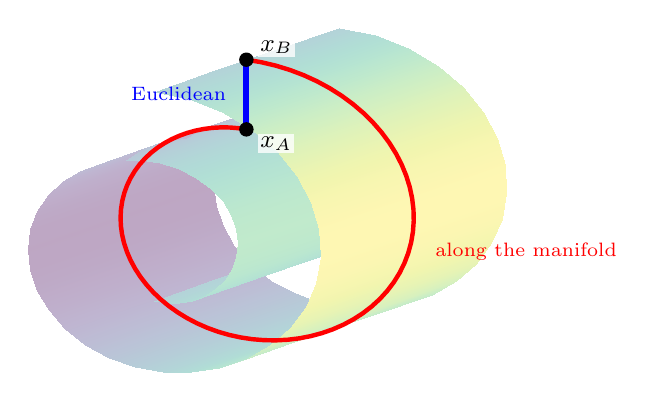
\begin{tikzpicture}
  \begin{axis}[width=9cm, height=7cm, view={25}{12}, axis lines=none, colormap/viridis,
      xmin=-15,xmax=15,ymin=0,ymax=10,zmin=-15,zmax=15, clip=false]
    \addplot3[surf, shader=interp, opacity=0.35, samples=50, samples y=4,
      domain=1.5*pi:4.5*pi, y domain=0:10, point meta=x]
      ({x*cos(deg(x))}, {y}, {x*sin(deg(x))});
    \addplot3[red, line width=1.6pt, samples=80, domain=2.5*pi:4.5*pi, variable=\t]
      ({\t*cos(deg(\t))}, {5}, {\t*sin(deg(\t))});
    \addplot3[blue, line width=2.2pt] coordinates {(0,5,{2.5*pi}) (0,5,{4.5*pi})};
\node[font=\scriptsize, blue, anchor=east] at (axis cs:-0.8,5,{3.5*pi}) {Euclidean};
\node[font=\scriptsize, red, anchor=west] at (axis cs:13.5,5,{-2}) {along the manifold};
    \addplot3[only marks, mark=*, mark size=2.4pt, black] coordinates {(0,5,{2.5*pi}) (0,5,{4.5*pi})};
    \node[font=\small, anchor=west, fill=white, inner sep=1pt, fill opacity=0.8, text opacity=1] at (axis cs:0.8,5,{2.5*pi-1.2}) {$\vect x_A$};
    \node[font=\small, anchor=west, fill=white, inner sep=1pt, fill opacity=0.8, text opacity=1] at (axis cs:0.8,5,{4.5*pi+1.2}) {$\vect x_B$};
  \end{axis}
\end{tikzpicture}
    \caption{The Swiss roll: a two-dimensional sheet rolled up in $\real^3$. The points $\vect x_A$ and $\vect x_B$ lie on neighboring layers. Their Euclidean distance (blue) is small, but their distance along the manifold (red, one full turn of the roll) is large. A nearest-neighbor graph built from densely sampled points connects only points that are close on the sheet, so the graph Laplacian measures smoothness along the manifold rather than in the ambient space.}
    \label{fig:swissroll}
  \end{figure}

\textbf{Intrinsic norm $\|\cdot\|_\text{I}$:}
  
  \begin{displaymath}
    \|f\|_\text{I}^2 = 
    \sum_{i=1}^m \sum_{j=i}^m w_{ij} \big( f(\vect{x}_i) - f(\vect{x}_j) \big)^2 = 
    \vect{f}^T \mat{L} \, \vect{f}
  \end{displaymath}
  A small example of $\mat W$, $\mat D$, $\mat L$ and of the intrinsic norm of a smooth and a non-smooth labeling is shown in Fig.~\ref{fig:lapsvm_graph}.

  \begin{figure}[htbp]
    \centering
    \begin{tikzpicture}[font=\small,
        nd/.style={circle,draw,thick,minimum size=5.5mm,inner sep=0pt},
        posnode/.style={nd,fill=red!35}, negnode/.style={nd,fill=blue!30}]
      % --- smooth labeling
      \begin{scope}
        \node[posnode] (a1) at (0,0) {1}; \node[posnode] (a2) at (1,0.7) {2}; \node[posnode] (a3) at (1,-0.7) {3};
        \node[negnode] (a4) at (2.6,-0.7) {4}; \node[negnode] (a5) at (3.6,0.7) {5}; \node[negnode] (a6) at (3.6,-0.7) {6};
        \draw[very thick] (a1)--(a2) (a1)--(a3) (a2)--(a3) (a4)--(a5) (a4)--(a6) (a5)--(a6);
        \draw[thin,dashed] (a3)--node[below,font=\scriptsize]{$0.2$}(a4);
        \node[align=center] at (1.8,-1.6) {$\vect f=(1,1,1,-1,-1,-1)^T$\\ $\vect f^T\mat L\vect f=0.2\cdot2^2=\mathbf{0.8}$};
      \end{scope}
      % --- rough labeling
      \begin{scope}[xshift=5.6cm]
        \node[posnode] (b1) at (0,0) {1}; \node[negnode] (b2) at (1,0.7) {2}; \node[posnode] (b3) at (1,-0.7) {3};
        \node[negnode] (b4) at (2.6,-0.7) {4}; \node[posnode] (b5) at (3.6,0.7) {5}; \node[negnode] (b6) at (3.6,-0.7) {6};
        \draw[very thick] (b1)--(b2) (b1)--(b3) (b2)--(b3) (b4)--(b5) (b4)--(b6) (b5)--(b6);
        \draw[thin,dashed] (b3)--node[below,font=\scriptsize]{$0.2$}(b4);
        \node[align=center] at (1.8,-1.6) {$\vect f=(1,-1,1,-1,1,-1)^T$\\ $\vect f^T\mat L\vect f=4\cdot 2^2+0.2\cdot2^2=\mathbf{16.8}$};
      \end{scope}
      % --- matrices
      \node[anchor=north,font=\footnotesize] (wd) at (4.6,-2.4) {$
        \mat W=\begin{pmatrix}0&1&1&0&0&0\\1&0&1&0&0&0\\1&1&0&0.2&0&0\\0&0&0.2&0&1&1\\0&0&0&1&0&1\\0&0&0&1&1&0\end{pmatrix},\quad
        \mat D=\mathrm{diag}(2,\,2,\,2.2,\,2.2,\,2,\,2),$};
      \node[anchor=north,font=\footnotesize] at ([yshift=-2pt]wd.south) {$
        \mat L=\mat D-\mat W=\begin{pmatrix}2&-1&-1&0&0&0\\-1&2&-1&0&0&0\\-1&-1&2.2&-0.2&0&0\\0&0&-0.2&2.2&-1&-1\\0&0&0&-1&2&-1\\0&0&0&-1&-1&2\end{pmatrix}$};
    \end{tikzpicture}
    \caption{Graph Laplacian and intrinsic norm for a toy graph with two clusters (edge weight $1$, thick) connected by one weak edge ($w_{34}=0.2$, dashed). Node colors show the values $f(\vect x_i)=\pm1$. Since $\vect f^T\mat L\vect f=\sum_{i<j}w_{ij}\big(f(\vect x_i)-f(\vect x_j)\big)^2$, every edge between differently colored nodes costs $w_{ij}\cdot 2^2$. Left: the labeling that is constant on each cluster only cuts the weak edge ($0.8$). Right: a labeling that alternates inside the clusters cuts four strong edges ($16.8$). Minimizing $\gamma_\text{I}\,\vect f^T\mat L\vect f$ therefore favors decision boundaries that pass through sparsely connected (low-density) regions.}
    \label{fig:lapsvm_graph}
  \end{figure}
    \textbf{Representer Theorem} (Kimeldorf and Wahba, 1970):    
  
  The solution $f^*$ of this optimization problem has the form:

  \begin{displaymath}
    f^*(\vect{x}) = \sum_{i=1}^m \beta_i^* \cdot k(\vect{x}_i, \vect{x}) + \beta_0^*
  \end{displaymath}
 
\subsection{Laplacian Support Vector Machines}\label{sec:lapsvm}
With the representer theorem, $\vect f=\mat K\vect\beta$, $\|f\|_\text{A}^2=\vect\beta^T\mat K\vect\beta$ and $\|f\|_\text{I}^2=\vect\beta^T\mat K\mat L\mat K\vect\beta$. With the hinge loss this gives the constrained \textbf{primal problem}
  \begin{eqnarray*}
    \mbox{minimize}   & & \sum_{i=1}^l \xi_i + \gamma_\text{A}\,\vect\beta^T\mat K\vect\beta + \gamma_\text{I}\,\vect\beta^T\mat K\mat L\mat K\vect\beta\\
    \mbox{subject to} & & y_i\Big(\sum_{j=1}^m \beta_j\, k(\vect x_i,\vect x_j)+\beta_0\Big)\ge 1-\xi_i,\quad \xi_i\ge 0,\quad i=1,\dots,l.
  \end{eqnarray*}
  (Compared with the soft-margin SVM, the slack weight is fixed to $1$ here; the trade-off is set by $\gamma_\text{A}$ and $\gamma_\text{I}$. Hence the box constraint below is $0\le\lambda_i\le1$ instead of $0\le\lambda_i\le\mu$.)
\textbf{Lagrange function $\mathcal L$} with multipliers $\lambda_i\ge0$ (margin constraints) and $\eta_i\ge0$ (constraints $\xi_i\ge0$):
  
  \begin{eqnarray*}
    \mathcal L(\vect\beta,\beta_0,\vect\xi,\vect\lambda,\vect\eta) 
    &=& \sum_{i=1}^l \xi_i +
        \frac{1}{2} \vect{\beta}^T (2 \gamma_\text{A} \mat{K} + 2 \gamma_\text{I} \mat{K}\mat{L}\mat{K}) \vect{\beta} -{} \\
    & & {}- \sum_{i=1}^l \lambda_i \left(y_i \Bigg(\sum_{j=1}^m \beta_j \, k(\vect{x}_i,\vect{x}_j) + \beta_0\Bigg) - 1 + \xi_i\right) -{} \\
    & & {}- \sum_{i=1}^l \eta_i \xi_i
  \end{eqnarray*}
     
    \textbf{KKT condition:} the gradient w.\,r.\,t. the primal variables $\vect{\beta}, \beta_0, \vect{\xi}$ has to vanish
   
  
  \begin{itemize}
    \item Partial derivative w.\,r.\,t. $\beta_0$:
      \begin{displaymath}
        \frac{\partial \mathcal L}{\partial \beta_0} \stackrel{!}{=} 0  \quad \Rightarrow \quad
        \sum_{i=1}^l \lambda_i y_i = 0
      \end{displaymath}
       
    \item Partial derivative w.\,r.\,t. $\xi_i$:
      \begin{displaymath}
        \frac{\partial \mathcal L}{\partial \xi_i} \stackrel{!}{=} 0  \quad \Rightarrow \quad
        1 - \lambda_i - \eta_i = 0 \quad \Rightarrow \quad
        0 \leq \lambda_i \leq 1
      \end{displaymath}
  \end{itemize}
  
    \textbf{Simplifying the Lagrangian using the two identities above:}
  
  {\small
    \begin{eqnarray*}
      \mathcal L(\vect{\beta}, \vect{\lambda}) 
      &=& \frac{1}{2} \vect{\beta}^T (2 \gamma_\text{A} \mat{K} + 2 \gamma_\text{I} \mat{K}\mat{L}\mat{K}) \vect{\beta} -{} \\
      & & {}- \sum_{i=1}^l \lambda_i \left(y_i \sum_{j=1}^m \beta_j k(\vect{x}_i,\vect{x}_j) - 1 \right) \qquad\text{(the $\beta_0$ term vanishes since $\textstyle\sum_i\lambda_iy_i=0$)} \\
      &=& \frac{1}{2} \vect{\beta}^T (2 \gamma_\text{A} \mat{K} + 2 \gamma_\text{I} \mat{K}\mat{L}\mat{K}) \vect{\beta} -
          \vect{\beta}^T \mat{K} \mat{J}_l^T \mat{Y} \vect{\lambda} +
          \sum_{i=1}^l \lambda_i
    \end{eqnarray*}
  }
  
  with $\mat{J}_l = [\mat{I}_l~\mat{0}] \in \real^{l\times m}$:
  \begin{itemize}
    \item identity matrix $\mat{I}_l \in \real^{l \times l}$
    \item rectangular matrix $\mat{0} \in \real^{l \times u}$ with all entries being 0
  \end{itemize}
  and diagonal matrix $\mat{Y} \in \real^{l \times l}$ composed by the $l$ class labels $y_i$\\
\textbf{Partial derivative w.\,r.\,t. $\vect{\beta}$:}
  
  \begin{eqnarray*}
    \frac{\partial \mathcal L}{\partial \vect{\beta}} \stackrel{!}{=} \vect{0} \\
    &\Rightarrow& 
    (2 \gamma_\text{A} \mat{K} + 2 \gamma_\text{I} \mat{K}\mat{L}\mat{K}) \vect{\beta} -
    \mat{K} \mat{J}_l^T \mat{Y} \vect{\lambda} = \vect{0}   \\
    &\Rightarrow& \text{(assuming $\mat K$ is invertible)} \\
    \vect{\beta} = (2 \gamma_\text{A} \mat{I}_m + 2 \gamma_\text{I} \mat{L}\mat{K})^{-1} 
    \mat{J}_l^T \mat{Y} \vect{\lambda}
  \end{eqnarray*}
   
    \textbf{Note:} direct relationship between parameters $\vect{\beta}$ and Lagrange multipliers $\vect{\lambda}$\\
   Substituting back in the Lagrangian expression leads to the dual problem
  \begin{displaymath}
    \max_{\vect\lambda}\ \sum_{i=1}^{l}\lambda_i - \frac{1}{2}\,\vect\lambda^T\mat Q\vect\lambda
    \quad\text{s.t.}\quad \sum_{i=1}^{l}\lambda_i y_i = 0,\ \ 0\le \lambda_i \le 1.
  \end{displaymath}
   where
  {\small
  \begin{displaymath}
    \mat{Q} = \mat{Y} \mat{J}_l \mat{K}
    (2 \gamma_\text{A} \mat{I}_m + 2 \gamma_\text{I} \mat{L}\mat{K})^{-1}
    \mat{J}_l^T \mat{Y}.
  \end{displaymath}
  }
 This is not to be memorized for the exam. 

 The decision boundaries in Figs.~\ref{fig:lapsvm_clock} and~\ref{fig:lapsvm_gammaI} were computed exactly this way: solve the dual for $\vect\lambda$, compute $\vect\beta$ from $\vect\lambda$, and obtain $\beta_0$ from a labeled point with $0<\lambda_i<1$, for which $y_if(\vect x_i)=1$. Figure~\ref{fig:lapsvm_gammaI} shows how the boundary changes with the weight $\gamma_\text{I}$ of the intrinsic term.

  \begin{figure}[htbp]
    \centering
    \begin{tikzpicture}
      \begin{groupplot}[group style={group size=2 by 2, horizontal sep=1.25cm, vertical sep=1.4cm}, width=4.35cm, height=4.35cm,
  axis equal image, xmin=-3.2,xmax=3.2,ymin=-3.2,ymax=3.2, xtick={-2,0,2}, ytick={-2,0,2},
  tick label style={font=\scriptsize}, title style={font=\small}]
        \nextgroupplot[title={$\gamma_\text{I}=0$}]
\addplot[only marks,mark=*,mark size=0.6pt,gray!60] coordinates {(-1.02,-0.08) (1.05,-0.34) (0.60,0.77) (0.89,-0.30) (-0.40,0.98) (-0.90,0.47) (0.50,-0.95) (-0.82,0.53) (-0.84,-0.27) (0.98,0.17) (0.02,-0.96) (-1.03,-0.25) (-0.49,0.89) (0.21,-0.84) (-0.30,0.85) (-1.03,0.31) (0.70,0.79) (-0.78,0.54) (0.29,0.96) (-0.08,1.03) (0.00,-1.04) (-0.20,1.05) (-1.02,0.09) (0.99,-0.12) (0.95,-0.23) (-0.17,-1.07) (-0.79,-0.21) (-0.17,0.97) (0.53,0.85) (0.87,-0.17) (-1.02,-0.10) (0.71,0.63) (-0.76,-0.75) (0.17,-0.98) (-0.80,-0.69) (0.95,-0.54) (1.00,0.25) (-0.91,-0.17) (-0.85,0.22) (1.05,0.44) (-0.63,-0.77) (0.57,-0.76) (-0.84,-0.56) (-0.06,0.98) (0.57,-0.90) (-1.00,-0.06) (-1.00,-0.07) (0.02,-0.94) (0.62,0.83) (0.39,-0.83) (-0.43,-0.96) (0.26,-1.09) (0.31,0.82) (0.26,-0.76) (0.38,0.98) (1.05,0.59) (0.56,-0.73) (0.58,-0.69) (0.75,-0.73) (-0.92,0.16) (-0.14,0.95) (0.97,0.04) (-0.64,-0.83) (-0.18,-0.95) (0.52,-0.88) (-0.20,0.97) (0.20,0.91) (-0.62,-0.75) (0.31,-0.87) (0.97,-0.23)};
\addplot[only marks,mark=*,mark size=0.6pt,gray!60] coordinates {(1.95,1.03) (-2.19,0.16) (0.53,2.21) (1.43,1.57) (-2.15,-0.08) (0.49,-2.17) (-0.56,1.92) (0.29,-2.43) (-2.12,-0.34) (1.27,1.73) (2.21,-0.50) (-1.79,1.27) (-0.58,1.98) (1.29,-1.85) (1.61,1.60) (-0.22,-2.15) (0.83,2.01) (-1.75,1.40) (0.24,2.11) (1.21,-1.88) (-1.71,1.41) (2.12,-0.34) (-1.47,-1.48) (-0.76,-2.05) (-2.11,-0.29) (-0.83,2.13) (-1.75,1.35) (2.11,-0.82) (0.67,2.11) (2.21,-0.16) (0.11,-2.13) (-1.43,1.74) (-1.48,-1.82) (-1.59,1.48) (-1.58,1.46) (-2.19,-0.05) (2.15,0.23) (-2.14,0.09) (2.18,-0.39) (-0.48,2.12) (-0.03,-2.31) (-2.06,0.77) (0.56,2.15) (1.88,-1.28) (2.16,0.23) (-0.76,2.19) (2.15,-0.01) (-0.16,2.13) (1.27,-1.76) (-1.73,-1.35) (0.72,-1.96) (-1.50,-1.60) (-1.34,1.57) (0.16,-2.31) (2.16,0.36) (-2.03,0.70) (-1.47,1.53) (-2.15,0.31) (1.52,1.57) (0.36,2.08) (-1.97,-0.81) (-1.66,1.42) (0.56,-2.08) (-1.80,-1.40) (1.47,-1.75) (-0.24,-2.19) (-1.80,-1.34) (-0.49,2.03) (0.46,-2.20) (-0.02,2.20) (1.99,1.02) (2.26,-0.54) (-1.95,-0.50) (0.33,-2.20) (-2.08,-0.39) (-1.72,-1.45) (2.05,0.44) (0.84,1.99) (-1.01,-1.97) (-2.03,-0.96) (1.20,1.85) (2.04,-0.63) (1.22,1.78) (-2.27,-0.15) (1.36,1.73) (-0.42,-2.02) (-0.37,2.24) (1.49,1.67) (2.18,0.65) (0.99,1.94) (0.81,2.12) (-2.06,-0.49) (-2.14,0.68) (2.08,-0.57) (2.16,-0.64) (0.66,-2.18) (-1.01,-1.89) (1.23,-1.82) (2.04,-0.83) (2.27,0.33) (1.66,1.53) (-1.34,1.62) (1.86,1.24) (-1.83,-1.32) (-0.15,2.36) (-0.19,2.06) (-0.51,2.09) (1.89,1.33) (-0.12,-2.09) (-1.23,-1.71) (-1.76,-1.39) (2.23,0.48) (-1.94,0.92) (-0.89,-2.06) (1.23,1.84) (-1.75,1.53) (2.18,0.27) (1.98,1.12) (0.45,2.08) (-1.88,1.12) (-2.13,0.50) (1.71,-1.52) (-0.91,2.05) (2.12,0.29) (1.04,-2.00) (2.09,0.86) (1.83,1.21) (2.12,-0.50) (0.05,-2.18) (-1.08,1.76)};
\addplot[only marks,mark=*,mark size=2.6pt,red,draw=black] coordinates {(0.00,1.00)};
\addplot[only marks,mark=square*,mark size=2.6pt,blue,draw=black] coordinates {(1.93,-1.05)};
\addplot[black, very thick] coordinates {(-2.41,-3.20) (-2.36,-3.15) (-2.28,-3.08) (-2.24,-3.04) (-2.16,-2.96) (-2.11,-2.92) (-2.04,-2.85) (-1.99,-2.80) (-1.92,-2.74) (-1.86,-2.68) (-1.80,-2.63) (-1.73,-2.56) (-1.68,-2.51) (-1.60,-2.44) (-1.56,-2.40) (-1.48,-2.33) (-1.43,-2.28) (-1.36,-2.21) (-1.31,-2.16) (-1.24,-2.10) (-1.18,-2.04) (-1.12,-1.99) (-1.05,-1.92) (-1.00,-1.87) (-0.92,-1.80) (-0.88,-1.76) (-0.80,-1.69) (-0.75,-1.64) (-0.68,-1.57) (-0.62,-1.52) (-0.56,-1.46) (-0.50,-1.40) (-0.44,-1.35) (-0.37,-1.28) (-0.32,-1.24) (-0.24,-1.16) (-0.20,-1.12) (-0.12,-1.05) (-0.07,-1.00) (0.00,-0.94) (0.06,-0.88) (0.12,-0.82) (0.19,-0.76) (0.24,-0.71) (0.31,-0.64) (0.36,-0.60) (0.44,-0.52) (0.48,-0.48) (0.56,-0.41) (0.61,-0.36) (0.68,-0.30) (0.74,-0.24) (0.80,-0.18) (0.87,-0.12) (0.92,-0.07) (0.99,0.00) (1.04,0.04) (1.12,0.12) (1.16,0.16) (1.24,0.23) (1.29,0.28) (1.36,0.34) (1.42,0.40) (1.48,0.46) (1.55,0.52) (1.60,0.57) (1.68,0.64) (1.72,0.68) (1.80,0.76) (1.85,0.80) (1.92,0.87) (1.97,0.92) (2.04,0.98) (2.10,1.04) (2.16,1.10) (2.23,1.16) (2.28,1.21) (2.36,1.28) (2.40,1.32) (2.48,1.40) (2.53,1.44) (2.60,1.51) (2.66,1.56) (2.72,1.62) (2.78,1.68) (2.84,1.74) (2.91,1.80) (2.96,1.85) (3.04,1.92) (3.08,1.96) (3.16,2.04)};
        \nextgroupplot[title={$\gamma_\text{I}=0.005$}]
\addplot[only marks,mark=*,mark size=0.6pt,gray!60] coordinates {(-1.02,-0.08) (1.05,-0.34) (0.60,0.77) (0.89,-0.30) (-0.40,0.98) (-0.90,0.47) (0.50,-0.95) (-0.82,0.53) (-0.84,-0.27) (0.98,0.17) (0.02,-0.96) (-1.03,-0.25) (-0.49,0.89) (0.21,-0.84) (-0.30,0.85) (-1.03,0.31) (0.70,0.79) (-0.78,0.54) (0.29,0.96) (-0.08,1.03) (0.00,-1.04) (-0.20,1.05) (-1.02,0.09) (0.99,-0.12) (0.95,-0.23) (-0.17,-1.07) (-0.79,-0.21) (-0.17,0.97) (0.53,0.85) (0.87,-0.17) (-1.02,-0.10) (0.71,0.63) (-0.76,-0.75) (0.17,-0.98) (-0.80,-0.69) (0.95,-0.54) (1.00,0.25) (-0.91,-0.17) (-0.85,0.22) (1.05,0.44) (-0.63,-0.77) (0.57,-0.76) (-0.84,-0.56) (-0.06,0.98) (0.57,-0.90) (-1.00,-0.06) (-1.00,-0.07) (0.02,-0.94) (0.62,0.83) (0.39,-0.83) (-0.43,-0.96) (0.26,-1.09) (0.31,0.82) (0.26,-0.76) (0.38,0.98) (1.05,0.59) (0.56,-0.73) (0.58,-0.69) (0.75,-0.73) (-0.92,0.16) (-0.14,0.95) (0.97,0.04) (-0.64,-0.83) (-0.18,-0.95) (0.52,-0.88) (-0.20,0.97) (0.20,0.91) (-0.62,-0.75) (0.31,-0.87) (0.97,-0.23)};
\addplot[only marks,mark=*,mark size=0.6pt,gray!60] coordinates {(1.95,1.03) (-2.19,0.16) (0.53,2.21) (1.43,1.57) (-2.15,-0.08) (0.49,-2.17) (-0.56,1.92) (0.29,-2.43) (-2.12,-0.34) (1.27,1.73) (2.21,-0.50) (-1.79,1.27) (-0.58,1.98) (1.29,-1.85) (1.61,1.60) (-0.22,-2.15) (0.83,2.01) (-1.75,1.40) (0.24,2.11) (1.21,-1.88) (-1.71,1.41) (2.12,-0.34) (-1.47,-1.48) (-0.76,-2.05) (-2.11,-0.29) (-0.83,2.13) (-1.75,1.35) (2.11,-0.82) (0.67,2.11) (2.21,-0.16) (0.11,-2.13) (-1.43,1.74) (-1.48,-1.82) (-1.59,1.48) (-1.58,1.46) (-2.19,-0.05) (2.15,0.23) (-2.14,0.09) (2.18,-0.39) (-0.48,2.12) (-0.03,-2.31) (-2.06,0.77) (0.56,2.15) (1.88,-1.28) (2.16,0.23) (-0.76,2.19) (2.15,-0.01) (-0.16,2.13) (1.27,-1.76) (-1.73,-1.35) (0.72,-1.96) (-1.50,-1.60) (-1.34,1.57) (0.16,-2.31) (2.16,0.36) (-2.03,0.70) (-1.47,1.53) (-2.15,0.31) (1.52,1.57) (0.36,2.08) (-1.97,-0.81) (-1.66,1.42) (0.56,-2.08) (-1.80,-1.40) (1.47,-1.75) (-0.24,-2.19) (-1.80,-1.34) (-0.49,2.03) (0.46,-2.20) (-0.02,2.20) (1.99,1.02) (2.26,-0.54) (-1.95,-0.50) (0.33,-2.20) (-2.08,-0.39) (-1.72,-1.45) (2.05,0.44) (0.84,1.99) (-1.01,-1.97) (-2.03,-0.96) (1.20,1.85) (2.04,-0.63) (1.22,1.78) (-2.27,-0.15) (1.36,1.73) (-0.42,-2.02) (-0.37,2.24) (1.49,1.67) (2.18,0.65) (0.99,1.94) (0.81,2.12) (-2.06,-0.49) (-2.14,0.68) (2.08,-0.57) (2.16,-0.64) (0.66,-2.18) (-1.01,-1.89) (1.23,-1.82) (2.04,-0.83) (2.27,0.33) (1.66,1.53) (-1.34,1.62) (1.86,1.24) (-1.83,-1.32) (-0.15,2.36) (-0.19,2.06) (-0.51,2.09) (1.89,1.33) (-0.12,-2.09) (-1.23,-1.71) (-1.76,-1.39) (2.23,0.48) (-1.94,0.92) (-0.89,-2.06) (1.23,1.84) (-1.75,1.53) (2.18,0.27) (1.98,1.12) (0.45,2.08) (-1.88,1.12) (-2.13,0.50) (1.71,-1.52) (-0.91,2.05) (2.12,0.29) (1.04,-2.00) (2.09,0.86) (1.83,1.21) (2.12,-0.50) (0.05,-2.18) (-1.08,1.76)};
\addplot[only marks,mark=*,mark size=2.6pt,red,draw=black] coordinates {(0.00,1.00)};
\addplot[only marks,mark=square*,mark size=2.6pt,blue,draw=black] coordinates {(1.93,-1.05)};
\addplot[black, very thick] coordinates {(-0.67,-3.20) (-0.72,-3.15) (-0.80,-3.08) (-0.84,-3.03) (-0.90,-2.96) (-0.96,-2.88) (-1.00,-2.81) (-1.04,-2.73) (-1.08,-2.64) (-1.10,-2.56) (-1.12,-2.48) (-1.13,-2.36) (-1.12,-2.26) (-1.09,-2.16) (-1.05,-2.08) (-1.00,-2.00) (-0.96,-1.96) (-0.89,-1.88) (-0.84,-1.84) (-0.76,-1.77) (-0.69,-1.72) (-0.64,-1.68) (-0.56,-1.62) (-0.48,-1.56) (-0.42,-1.52) (-0.36,-1.48) (-0.28,-1.42) (-0.20,-1.36) (-0.15,-1.32) (-0.08,-1.26) (-0.01,-1.20) (0.04,-1.16) (0.12,-1.08) (0.16,-1.04) (0.24,-0.96) (0.28,-0.91) (0.35,-0.84) (0.40,-0.78) (0.46,-0.72) (0.52,-0.65) (0.56,-0.60) (0.64,-0.52) (0.68,-0.47) (0.74,-0.40) (0.80,-0.34) (0.85,-0.28) (0.92,-0.21) (0.96,-0.16) (1.04,-0.08) (1.08,-0.03) (1.15,0.04) (1.20,0.10) (1.25,0.16) (1.32,0.24) (1.36,0.29) (1.42,0.36) (1.48,0.44) (1.52,0.50) (1.56,0.56) (1.62,0.64) (1.67,0.72) (1.71,0.80) (1.75,0.88) (1.79,0.96) (1.82,1.04) (1.86,1.12) (1.89,1.20) (1.92,1.28) (1.96,1.36) (2.00,1.45) (2.04,1.52) (2.09,1.60) (2.16,1.68) (2.20,1.72) (2.28,1.77) (2.36,1.81) (2.48,1.84) (2.56,1.85) (2.68,1.84) (2.76,1.83) (2.88,1.80) (2.96,1.77) (3.04,1.74) (3.12,1.69) (3.19,1.64)};
\addplot[black, very thick] coordinates {(3.20,-2.86) (3.18,-2.88) (3.16,-2.89) (3.12,-2.92) (3.11,-2.92) (3.08,-2.94) (3.05,-2.96) (3.04,-2.96) (3.00,-2.99) (2.98,-3.00) (2.96,-3.01) (2.92,-3.03) (2.90,-3.04) (2.88,-3.05) (2.84,-3.07) (2.81,-3.08) (2.80,-3.09) (2.76,-3.11) (2.72,-3.12) (2.72,-3.12) (2.68,-3.14) (2.64,-3.16) (2.63,-3.16) (2.60,-3.17) (2.56,-3.19) (2.52,-3.20)};
        \nextgroupplot[title={$\gamma_\text{I}=0.05$}]
\addplot[only marks,mark=*,mark size=0.6pt,gray!60] coordinates {(-1.02,-0.08) (1.05,-0.34) (0.60,0.77) (0.89,-0.30) (-0.40,0.98) (-0.90,0.47) (0.50,-0.95) (-0.82,0.53) (-0.84,-0.27) (0.98,0.17) (0.02,-0.96) (-1.03,-0.25) (-0.49,0.89) (0.21,-0.84) (-0.30,0.85) (-1.03,0.31) (0.70,0.79) (-0.78,0.54) (0.29,0.96) (-0.08,1.03) (0.00,-1.04) (-0.20,1.05) (-1.02,0.09) (0.99,-0.12) (0.95,-0.23) (-0.17,-1.07) (-0.79,-0.21) (-0.17,0.97) (0.53,0.85) (0.87,-0.17) (-1.02,-0.10) (0.71,0.63) (-0.76,-0.75) (0.17,-0.98) (-0.80,-0.69) (0.95,-0.54) (1.00,0.25) (-0.91,-0.17) (-0.85,0.22) (1.05,0.44) (-0.63,-0.77) (0.57,-0.76) (-0.84,-0.56) (-0.06,0.98) (0.57,-0.90) (-1.00,-0.06) (-1.00,-0.07) (0.02,-0.94) (0.62,0.83) (0.39,-0.83) (-0.43,-0.96) (0.26,-1.09) (0.31,0.82) (0.26,-0.76) (0.38,0.98) (1.05,0.59) (0.56,-0.73) (0.58,-0.69) (0.75,-0.73) (-0.92,0.16) (-0.14,0.95) (0.97,0.04) (-0.64,-0.83) (-0.18,-0.95) (0.52,-0.88) (-0.20,0.97) (0.20,0.91) (-0.62,-0.75) (0.31,-0.87) (0.97,-0.23)};
\addplot[only marks,mark=*,mark size=0.6pt,gray!60] coordinates {(1.95,1.03) (-2.19,0.16) (0.53,2.21) (1.43,1.57) (-2.15,-0.08) (0.49,-2.17) (-0.56,1.92) (0.29,-2.43) (-2.12,-0.34) (1.27,1.73) (2.21,-0.50) (-1.79,1.27) (-0.58,1.98) (1.29,-1.85) (1.61,1.60) (-0.22,-2.15) (0.83,2.01) (-1.75,1.40) (0.24,2.11) (1.21,-1.88) (-1.71,1.41) (2.12,-0.34) (-1.47,-1.48) (-0.76,-2.05) (-2.11,-0.29) (-0.83,2.13) (-1.75,1.35) (2.11,-0.82) (0.67,2.11) (2.21,-0.16) (0.11,-2.13) (-1.43,1.74) (-1.48,-1.82) (-1.59,1.48) (-1.58,1.46) (-2.19,-0.05) (2.15,0.23) (-2.14,0.09) (2.18,-0.39) (-0.48,2.12) (-0.03,-2.31) (-2.06,0.77) (0.56,2.15) (1.88,-1.28) (2.16,0.23) (-0.76,2.19) (2.15,-0.01) (-0.16,2.13) (1.27,-1.76) (-1.73,-1.35) (0.72,-1.96) (-1.50,-1.60) (-1.34,1.57) (0.16,-2.31) (2.16,0.36) (-2.03,0.70) (-1.47,1.53) (-2.15,0.31) (1.52,1.57) (0.36,2.08) (-1.97,-0.81) (-1.66,1.42) (0.56,-2.08) (-1.80,-1.40) (1.47,-1.75) (-0.24,-2.19) (-1.80,-1.34) (-0.49,2.03) (0.46,-2.20) (-0.02,2.20) (1.99,1.02) (2.26,-0.54) (-1.95,-0.50) (0.33,-2.20) (-2.08,-0.39) (-1.72,-1.45) (2.05,0.44) (0.84,1.99) (-1.01,-1.97) (-2.03,-0.96) (1.20,1.85) (2.04,-0.63) (1.22,1.78) (-2.27,-0.15) (1.36,1.73) (-0.42,-2.02) (-0.37,2.24) (1.49,1.67) (2.18,0.65) (0.99,1.94) (0.81,2.12) (-2.06,-0.49) (-2.14,0.68) (2.08,-0.57) (2.16,-0.64) (0.66,-2.18) (-1.01,-1.89) (1.23,-1.82) (2.04,-0.83) (2.27,0.33) (1.66,1.53) (-1.34,1.62) (1.86,1.24) (-1.83,-1.32) (-0.15,2.36) (-0.19,2.06) (-0.51,2.09) (1.89,1.33) (-0.12,-2.09) (-1.23,-1.71) (-1.76,-1.39) (2.23,0.48) (-1.94,0.92) (-0.89,-2.06) (1.23,1.84) (-1.75,1.53) (2.18,0.27) (1.98,1.12) (0.45,2.08) (-1.88,1.12) (-2.13,0.50) (1.71,-1.52) (-0.91,2.05) (2.12,0.29) (1.04,-2.00) (2.09,0.86) (1.83,1.21) (2.12,-0.50) (0.05,-2.18) (-1.08,1.76)};
\addplot[only marks,mark=*,mark size=2.6pt,red,draw=black] coordinates {(0.00,1.00)};
\addplot[only marks,mark=square*,mark size=2.6pt,blue,draw=black] coordinates {(1.93,-1.05)};
\addplot[black, very thick] coordinates {(-1.09,-3.20) (-1.18,-3.12) (-1.26,-3.04) (-1.33,-2.96) (-1.40,-2.88) (-1.48,-2.77) (-1.55,-2.68) (-1.60,-2.60) (-1.68,-2.48) (-1.73,-2.40) (-1.80,-2.28) (-1.84,-2.19) (-1.88,-2.08) (-1.92,-1.93) (-1.93,-1.80) (-1.90,-1.68) (-1.83,-1.60) (-1.69,-1.56) (-1.60,-1.56) (-1.44,-1.58) (-1.32,-1.61) (-1.16,-1.63) (-1.04,-1.65) (-0.88,-1.67) (-0.76,-1.68) (-0.60,-1.69) (-0.44,-1.69) (-0.28,-1.68) (-0.16,-1.67) (0.00,-1.64) (0.12,-1.61) (0.24,-1.57) (0.36,-1.52) (0.44,-1.48) (0.56,-1.41) (0.64,-1.34) (0.72,-1.27) (0.80,-1.17) (0.87,-1.08) (0.92,-1.00) (0.99,-0.88) (1.04,-0.79) (1.09,-0.68) (1.15,-0.56) (1.20,-0.47) (1.25,-0.36) (1.31,-0.24) (1.36,-0.12) (1.40,-0.02) (1.44,0.08) (1.48,0.20) (1.52,0.34) (1.55,0.48) (1.57,0.60) (1.58,0.76) (1.58,0.92) (1.56,1.07) (1.53,1.20) (1.49,1.32) (1.44,1.43) (1.39,1.52) (1.32,1.64) (1.26,1.72) (1.20,1.81) (1.12,1.92) (1.07,2.00) (1.01,2.12) (1.03,2.28) (1.12,2.36) (1.20,2.40) (1.32,2.45) (1.46,2.48) (1.60,2.50) (1.76,2.50) (1.92,2.49) (2.04,2.47) (2.16,2.44) (2.28,2.40) (2.40,2.36) (2.52,2.31) (2.64,2.26) (2.75,2.20) (2.84,2.15) (2.95,2.08) (3.04,2.02) (3.12,1.95)};
\addplot[black, very thick] coordinates {(3.20,-2.49) (3.17,-2.52) (3.16,-2.52) (3.12,-2.55) (3.11,-2.56) (3.08,-2.58) (3.05,-2.60) (3.04,-2.61) (3.00,-2.63) (2.99,-2.64) (2.96,-2.66) (2.92,-2.68) (2.92,-2.68) (2.88,-2.70) (2.85,-2.72) (2.84,-2.73) (2.80,-2.75) (2.78,-2.76) (2.76,-2.77) (2.72,-2.79) (2.71,-2.80) (2.68,-2.82) (2.64,-2.84) (2.64,-2.84) (2.60,-2.86) (2.57,-2.88) (2.56,-2.89) (2.52,-2.91) (2.50,-2.92) (2.48,-2.94) (2.44,-2.96) (2.44,-2.96) (2.40,-2.99) (2.39,-3.00) (2.36,-3.02) (2.33,-3.04) (2.32,-3.05) (2.28,-3.08) (2.28,-3.08) (2.24,-3.11) (2.23,-3.12) (2.20,-3.14) (2.18,-3.16) (2.16,-3.18) (2.13,-3.20)};
        \nextgroupplot[title={$\gamma_\text{I}=1$}]
\addplot[only marks,mark=*,mark size=0.6pt,gray!60] coordinates {(-1.02,-0.08) (1.05,-0.34) (0.60,0.77) (0.89,-0.30) (-0.40,0.98) (-0.90,0.47) (0.50,-0.95) (-0.82,0.53) (-0.84,-0.27) (0.98,0.17) (0.02,-0.96) (-1.03,-0.25) (-0.49,0.89) (0.21,-0.84) (-0.30,0.85) (-1.03,0.31) (0.70,0.79) (-0.78,0.54) (0.29,0.96) (-0.08,1.03) (0.00,-1.04) (-0.20,1.05) (-1.02,0.09) (0.99,-0.12) (0.95,-0.23) (-0.17,-1.07) (-0.79,-0.21) (-0.17,0.97) (0.53,0.85) (0.87,-0.17) (-1.02,-0.10) (0.71,0.63) (-0.76,-0.75) (0.17,-0.98) (-0.80,-0.69) (0.95,-0.54) (1.00,0.25) (-0.91,-0.17) (-0.85,0.22) (1.05,0.44) (-0.63,-0.77) (0.57,-0.76) (-0.84,-0.56) (-0.06,0.98) (0.57,-0.90) (-1.00,-0.06) (-1.00,-0.07) (0.02,-0.94) (0.62,0.83) (0.39,-0.83) (-0.43,-0.96) (0.26,-1.09) (0.31,0.82) (0.26,-0.76) (0.38,0.98) (1.05,0.59) (0.56,-0.73) (0.58,-0.69) (0.75,-0.73) (-0.92,0.16) (-0.14,0.95) (0.97,0.04) (-0.64,-0.83) (-0.18,-0.95) (0.52,-0.88) (-0.20,0.97) (0.20,0.91) (-0.62,-0.75) (0.31,-0.87) (0.97,-0.23)};
\addplot[only marks,mark=*,mark size=0.6pt,gray!60] coordinates {(1.95,1.03) (-2.19,0.16) (0.53,2.21) (1.43,1.57) (-2.15,-0.08) (0.49,-2.17) (-0.56,1.92) (0.29,-2.43) (-2.12,-0.34) (1.27,1.73) (2.21,-0.50) (-1.79,1.27) (-0.58,1.98) (1.29,-1.85) (1.61,1.60) (-0.22,-2.15) (0.83,2.01) (-1.75,1.40) (0.24,2.11) (1.21,-1.88) (-1.71,1.41) (2.12,-0.34) (-1.47,-1.48) (-0.76,-2.05) (-2.11,-0.29) (-0.83,2.13) (-1.75,1.35) (2.11,-0.82) (0.67,2.11) (2.21,-0.16) (0.11,-2.13) (-1.43,1.74) (-1.48,-1.82) (-1.59,1.48) (-1.58,1.46) (-2.19,-0.05) (2.15,0.23) (-2.14,0.09) (2.18,-0.39) (-0.48,2.12) (-0.03,-2.31) (-2.06,0.77) (0.56,2.15) (1.88,-1.28) (2.16,0.23) (-0.76,2.19) (2.15,-0.01) (-0.16,2.13) (1.27,-1.76) (-1.73,-1.35) (0.72,-1.96) (-1.50,-1.60) (-1.34,1.57) (0.16,-2.31) (2.16,0.36) (-2.03,0.70) (-1.47,1.53) (-2.15,0.31) (1.52,1.57) (0.36,2.08) (-1.97,-0.81) (-1.66,1.42) (0.56,-2.08) (-1.80,-1.40) (1.47,-1.75) (-0.24,-2.19) (-1.80,-1.34) (-0.49,2.03) (0.46,-2.20) (-0.02,2.20) (1.99,1.02) (2.26,-0.54) (-1.95,-0.50) (0.33,-2.20) (-2.08,-0.39) (-1.72,-1.45) (2.05,0.44) (0.84,1.99) (-1.01,-1.97) (-2.03,-0.96) (1.20,1.85) (2.04,-0.63) (1.22,1.78) (-2.27,-0.15) (1.36,1.73) (-0.42,-2.02) (-0.37,2.24) (1.49,1.67) (2.18,0.65) (0.99,1.94) (0.81,2.12) (-2.06,-0.49) (-2.14,0.68) (2.08,-0.57) (2.16,-0.64) (0.66,-2.18) (-1.01,-1.89) (1.23,-1.82) (2.04,-0.83) (2.27,0.33) (1.66,1.53) (-1.34,1.62) (1.86,1.24) (-1.83,-1.32) (-0.15,2.36) (-0.19,2.06) (-0.51,2.09) (1.89,1.33) (-0.12,-2.09) (-1.23,-1.71) (-1.76,-1.39) (2.23,0.48) (-1.94,0.92) (-0.89,-2.06) (1.23,1.84) (-1.75,1.53) (2.18,0.27) (1.98,1.12) (0.45,2.08) (-1.88,1.12) (-2.13,0.50) (1.71,-1.52) (-0.91,2.05) (2.12,0.29) (1.04,-2.00) (2.09,0.86) (1.83,1.21) (2.12,-0.50) (0.05,-2.18) (-1.08,1.76)};
\addplot[only marks,mark=*,mark size=2.6pt,red,draw=black] coordinates {(0.00,1.00)};
\addplot[only marks,mark=square*,mark size=2.6pt,blue,draw=black] coordinates {(1.93,-1.05)};
\addplot[black, very thick] coordinates {(-0.12,-1.60) (0.04,-1.61) (0.20,-1.60) (0.32,-1.58) (0.44,-1.55) (0.56,-1.50) (0.68,-1.44) (0.76,-1.39) (0.87,-1.32) (0.96,-1.25) (1.04,-1.18) (1.12,-1.10) (1.20,-1.00) (1.26,-0.92) (1.32,-0.82) (1.38,-0.72) (1.43,-0.60) (1.47,-0.48) (1.50,-0.36) (1.53,-0.24) (1.55,-0.08) (1.56,0.08) (1.56,0.20) (1.56,0.32) (1.55,0.48) (1.52,0.62) (1.48,0.76) (1.44,0.85) (1.38,0.96) (1.32,1.04) (1.24,1.13) (1.16,1.20) (1.06,1.28) (0.96,1.34) (0.87,1.40) (0.76,1.46) (0.64,1.52) (0.54,1.56) (0.42,1.60) (0.28,1.64) (0.16,1.66) (0.00,1.67) (-0.16,1.67) (-0.32,1.64) (-0.44,1.61) (-0.56,1.57) (-0.68,1.52) (-0.76,1.48) (-0.88,1.41) (-0.96,1.36) (-1.06,1.28) (-1.16,1.20) (-1.24,1.12) (-1.31,1.04) (-1.37,0.96) (-1.44,0.87) (-1.50,0.76) (-1.56,0.65) (-1.60,0.55) (-1.64,0.42) (-1.67,0.28) (-1.68,0.12) (-1.67,-0.04) (-1.64,-0.20) (-1.61,-0.32) (-1.58,-0.44) (-1.53,-0.56) (-1.48,-0.68) (-1.44,-0.76) (-1.37,-0.88) (-1.32,-0.96) (-1.24,-1.06) (-1.16,-1.15) (-1.08,-1.22) (-1.00,-1.28) (-0.88,-1.36) (-0.80,-1.41) (-0.68,-1.46) (-0.56,-1.50) (-0.44,-1.54) (-0.32,-1.57) (-0.16,-1.60)};
      \end{groupplot}
    \end{tikzpicture}
    \caption{Influence of the intrinsic regularization weight $\gamma_\text{I}$ (same data and parameters as Fig.~\ref{fig:lapsvm_clock}, $\gamma_\text{A}=1/32$ fixed). For $\gamma_\text{I}=0$ the classifier is an ordinary SVM trained on two points. With increasing $\gamma_\text{I}$, cutting through densely connected regions of the graph becomes more and more expensive, and the boundary is pushed out of the rings into the low-density gap between them.}
    \label{fig:lapsvm_gammaI}
  \end{figure}
 
\subsection{Lessons Learned}
   \textbf{Laplacian SVM:}
  
  \begin{itemize}
    \item Ongoing research topic   
    \item Extension of the Kernel SVM   
    \item Additional regularization term   
    \item Derivation of the dual problem
  \end{itemize}
 
  \newpage 
\section{The Expectation Maximization Algorithm}\autocite{dempster1977,bishop2006,hastie2009}

An important chapter for the exam. understand the steps, and if possible do the exercise to understand better. 

\subsection{Parameter Estimation}
\textbf{Goal:} Derivation of a parameter estimation technique that can deal with high-dimensional parameter spaces and with latent, hidden, or incomplete data.
  
  Two parameter estimation techniques are known from statistics. In \textbf{maximum likelihood estimation (ML estimation)}, all observations are assumed to be mutually statistically independent; the observations are kept fixed, and the (log-)likelihood function is optimized with respect to the parameters. In \textbf{maximum a-posteriori estimation (MAP estimation)}, the probability density function $p(\vect{\theta})$ of the parameters to be estimated is additionally assumed to be known, and the posterior of the parameters given the observations is maximized.
  
  Let $X$ be the observed random variable and $\p$ the parameter set. The estimates of $\p$ are denoted by $\hatp$.
  Let $x$ be a realization (observed value) of $X$.
%
  The \textbf{ML estimate} is
  \begin{displaymath}
    \hatp= \argmax_{\p}\ p(x; \p) = \argmax_{\p}\ \log p(x; \p),
  \end{displaymath}
  and the \textbf{MAP estimate} is
      {\small
        \begin{eqnarray*}
          \hatp &=& \argmax_{\p}\ p(\p|{x})\\
                &=& \argmax_{\p}\ \frac{p(\p)\,p(x|\p)}{\int p(\p')\,p(x|\p')\,\mathsf{d}\p'}\\
                &=& \argmax_{\p}\ \log p(\p) + \log p(x|\p)
        \end{eqnarray*}
      }
  Here $\p$ is considered as a random variable and its probability density function $p(\p)$ is known. The denominator (the evidence) does not depend on $\p$ and can be dropped in the maximization.
     

  \subsubsection{ML Estimation: Example}

    Let us assume a Gaussian distributed random vector:
%
    \begin{displaymath}
      p(\vect{x};\vect{\mu}, \mat{\Sigma}) = \frac{1}{\sqrt{\det(2\pi\mat{\Sigma})}}
        e^{-\frac{1}{2}(\vect{x}-\vect{\mu})^T \mat{\Sigma}^{-1} (\vect{x}-\vect{\mu})}  
    \end{displaymath}
%    
    \begin{itemize}
      \item We observe the random vectors $\vect{x}_1, \vect{x}_2, \dots, \vect{x}_m$ (training data).  
      \item Based on these training data, we have to estimate the mean vector $\vect{\mu}$ and the covariance matrix $\mat{\Sigma}$.
    \end{itemize}

    \small
    The ML estimator assumes   \textbf{mutually independent observations} and optimizes the pdf for the given set of training data:
%
    {\footnotesize
      \begin{eqnarray*}
        \{\hat{\vect{\mu}}, \hat{\mat{\Sigma}}\}
          &=& \argmax_{\vect{\mu},\mat{\Sigma}}\ \prod_{i=1}^m p(\vect{x}_i;\vect{\mu}, \mat{\Sigma}) \\   
          &=& \argmax_{\vect{\mu},\mat{\Sigma}}\ \sum_{i=1}^m \log p(\vect{x}_i;\vect{\mu}, \mat{\Sigma}) \\  
          &=& \argmax_{\vect{\mu},\mat{\Sigma}} L(\vect{x}_1, \vect{x}_2, \dots, \vect{x}_m; \vect{\mu}, \mat{\Sigma})  
      \end{eqnarray*}
    }
%
    where the   \textbf{log-likelihood function} is defined by
%
    \begin{displaymath}
        L:= L(\vect{x}_1, \vect{x}_2, \dots, \vect{x}_m; \vect{\mu}, \mat{\Sigma}) =
        \sum_{i=1}^m \log p(\vect{x}_i;\vect{\mu}, \mat{\Sigma})
      \end{displaymath}\\
    \textbf{Necessary conditions} for the estimation of the parameters are:\\
       \begin{displaymath}
         \frac{\partial L}{\partial \vect{\mu}} \stackrel{!}{=} \vect{0} 
         \quad \quad \mbox{and} \quad \quad
         \frac{\partial L}{\partial \mat{\Sigma}} \stackrel{!}{=} \mat{0}  
       \end{displaymath}\\
     Now we get for the mean vector:\\%  
       \begin{displaymath}
         \frac{\partial L}{\partial \vect{\mu}} = 
         \sum_{i=1}^m \mat{\Sigma}^{-1}(\vect x_i-\vect{\mu}) \stackrel{!}{=} 
         \vect{0}  
       \end{displaymath}\\
     and thus the   \textbf{ML estimate for the mean vector} meets our expectation:\\
      \begin{displaymath}
         \vect{\hat{\mu}} = \frac{1}{m}\sum_{i=1}^m \vect{x}_i
      \end{displaymath}\\
   \small
    Along the same lines, we get the   \textbf{estimator of the covariance matrix} by computation of the zero crossings of the partial derivatives w.\,r.\,t.\ the components of the covariance matrix:
 
    \begin{displaymath}
      \hat{\mat{\Sigma}} = \frac{1}{m} \sum_{i=1}^m (\vect x_i-\hat{\vect{\mu}})
                                                    (\vect x_i-\hat{\vect{\mu}})^T
    \end{displaymath}
  
\subsection{Gaussian Mixture Models}

recommend to implement this exercise. theory is important for the exam. So far, we have considered parameter estimation for statistical models with:  
  \begin{itemize}
    \item one class-dependent distribution component  
    \item uni- or multivariate feature vectors  
    \item the type was mostly Gaussian (normally distributed features)
  \end{itemize}
   
  Now we extend this model by representing the observations with a set of $K$ multivariate Gaussian distributions:\\
 \textbf{Problem description:} \\
  
  Given $m$ feature vectors in an $d$ dimensional space, find a set of $K$ multivariate Gaussian distributions that best represent the observations. GMMs are an example of   \textbf{\emph{unsupervised learning}} (clustering, density estimation):  

  \begin{itemize}
    \item It is not known which feature vectors are generated by which of the $K$ Gaussians  
    \item The desired output is, for each feature vector, an estimate of the probability that it is generated by distribution $k$
  \end{itemize}
     
 \textbf{GMM parameter estimation:} parameters $\vect\theta=\{\pi_k,\vect\mu_k,\mat\Sigma_k\}_{k=1}^K$
%  
  \begin{eqnarray*}
    \vect\mu_k    &\phantom{=}& \mbox{the $K$ means} \\
    \mat\Sigma_k &\phantom{=}& \mbox{the $K$ covariance matrices of size $d \times d$} \\
    \pi_k          &\phantom{=}& \mbox{mixture weights, with $\pi_k\ge 0$ and $\sum_k \pi_k=1$} \\
    z_i          &\phantom{=}& \mbox{hidden component label of $\vect x_i$, $z_i\in\{1,\dots,K\}$}\\
    \gamma_{ik}       &\phantom{=}& p(z_i=k\mid \vect x_i;\hat{\vect\theta})\ \mbox{(responsibility)}
  \end{eqnarray*}
    \textbf{Additional estimates:}
%  
  \begin{eqnarray*}
    p(\vect x;\vect\theta) &\phantom{=}& \mbox{density of observing a feature vector $\vect x$} \\
    \ell(\vect\theta)         &\phantom{=}& \mbox{overall log-likelihood function of the parameter set}
  \end{eqnarray*}
     
  \subsubsection{GMM -- Expectation}
  
  The key to the estimation problem is the \textbf{overall log-likelihood objective function $\ell(\vect\theta)$}:
  \begin{displaymath}
    \ell(\vect\theta) = \sum_{i = 1}^{m} \log p(\vect x_i;\vect\theta)
  \end{displaymath}
  
  Split $p(\vect x_i;\vect\theta)$ into its contributions from the $K$ Gaussians:
  \begin{displaymath}
    p(\vect x_i;\vect\theta) = \sum_{k=1}^{K} \pi_k \, {\mathcal N}(\vect x_i; \vect \mu_k, \mat \Sigma_k)
  \end{displaymath}

  Individual probabilities for the $K$ contributions (responsibilities):
  \begin{displaymath}
    \gamma_{ik} = p(z_i=k\mid\vect x_i;\hat{\vect\theta}) = \frac{ \hat\pi_k\,{\mathcal N}(\vect x_i; \hat{\vect \mu}_k, \hat{\mat \Sigma}_k)}{p(\vect x_i;\hat{\vect\theta})}
  \end{displaymath}
     
 \subsubsection{GMM -- Maximization}
  
    \textbf{Problem:} How do we get $\vect \mu_k, \mat \Sigma_k$ and $\pi_k$?  

  \begin{itemize}
    \item Similar to the ML estimate for the Gaussian, we maximize the log-likelihood by deriving w.\,r.\,t.\ the unknowns.     
    \item The   \textbf{ML estimates} are:
      \begin{eqnarray*}
        \hat{\vect \mu}_k 
          &=& \frac{\sum_i \gamma_{ik} \vect x_i}{\sum_i \gamma_{ik}} \\
        \hat{\mat \Sigma}_k 
          &=& \frac{\sum_i \gamma_{ik} (\vect x_i - \hat{\vect \mu}_k)(\vect x_i - \hat{\vect \mu}_k)^T}{\sum_i \gamma_{ik}} \\
        \hat{\pi}_k 
          &=& \frac{1}{m} \sum_{i=1}^m \gamma_{ik}
      \end{eqnarray*}
  \end{itemize}

  \paragraph{Where the M-step updates come from (sketch).}
  Using responsibilities $\gamma_{ik}=p(z_i=k\mid\vect x_i;\hat{\vect\theta})$ from the E-step, the stationarity conditions of the log-likelihood yield the closed-form updates.

  \textbf{Mean $\vect\mu_k$:}
  {\small
  \begin{align*}
    \frac{\partial \ell}{\partial \vect\mu_k}
      &= \sum_{i=1}^m
          \frac{\pi_k\,\mathcal N(\vect x_i;\vect\mu_k,\mat\Sigma_k)}{\sum_{l} \pi_l\,\mathcal N(\vect x_i;\vect\mu_l,\mat\Sigma_l)}\,\mat\Sigma_k^{-1}(\vect x_i-\vect\mu_k)
       = \sum_{i=1}^m \gamma_{ik}\,\mat\Sigma_k^{-1}(\vect x_i-\vect\mu_k)
       ~\stackrel{!}{=}~ \vect 0\\
    \Rightarrow\quad \hat{\vect\mu}_k &= \frac{\sum_i \gamma_{ik}\,\vect x_i}{\sum_i \gamma_{ik}}\,.
  \end{align*}
  }

  \textbf{Covariance $\mat\Sigma_k$:} same as the single-Gaussian ML estimate, but each sample is weighted by $\gamma_{ik}$:
  {\small
  \[
    \hat{\mat\Sigma}_k = \frac{\sum_i \gamma_{ik}(\vect x_i-\hat{\vect\mu}_k)(\vect x_i-\hat{\vect\mu}_k)^{T}}{\sum_i \gamma_{ik}}\,.
  \]
  }

  \textbf{Mixture weights $\pi_k$:} enforce $\sum_k \pi_k=1$ via a Lagrangian $\mathcal L = \ell(\vect\theta)+\nu(\sum_k \pi_k-1)$ and set $\partial\mathcal L/\partial \pi_k=0$ (see Sec.~\emph{Constrained Optimization} below),
  which yields $\hat \pi_k=\tfrac{1}{m}\sum_i \gamma_{ik}$.

  \subsubsection*{GMM Parameter Estimation}
    \textbf{Observations:}

  \begin{itemize}
    \item If we know the values for the parameters ($\vect \mu_k, \mat \Sigma_k, \pi_k$), we can compute the expectations (\textbf {E-step}).     
    \item Once we have the expectations we can compute improved values for the parameters (\textbf {M-step}).
  \end{itemize}
     
  We have found an   \textbf{iterative solution scheme} for the nonlinear GMM parameter estimation problem:

  \begin{itemize}
    \item \emph{Right at} the ML solution both E- and M-step relations hold.   
    \item The ML parameters are a stationary point for the E- and M-step.   
    \item Starting from any parameter values, an iteration of the E-step combined with an M-step will not decrease $\ell$.
  \end{itemize}
\textbf{EM algorithm for GMM parameter estimation:}\\
refer to slides\\

  \begin{centernss}
    \begin{struktogramm}(100,50)
      \assign{Initialization: $\vect \mu_k^{(0)}, \mat \Sigma_k^{(0)}, \pi_k^{(0)}$}
      \assign{$j \gets 0$}
      \until{$\left|\ell^{(j+1)}-\ell^{(j)}\right| < \varepsilon$}
        \assign{\textbf{Expectation step}: compute new values for $\gamma_{ik}, \ell$}
        \assign{\textbf{Maximization step}: compute $\vect \mu_k^{(j+1)}, \mat \Sigma_k^{(j+1)}, \pi_k^{(j+1)}$}
        \assign{$j \gets j+1$}
      \untilend
      \assign{Output: estimates $\hat{\vect \mu}_k, \hat{\mat \Sigma}_k, \hat{\pi}_k$}
    \end{struktogramm}
  \end{centernss}

\subsection{Missing Information Principle}

  A colloquial formulation of the   \textbf{missing information principle (MIP)} is as simple as:  observable information $=$ complete information $-$ hidden information

     
\textbf{Mathematical formalization of the MIP:}
  Let $X$ be the observable random variable, $Z$ the hidden random variable, and $\p$ the parameter set.
   
  The joint density of the events $x$ (observation) and $z$ (hidden) is:
  \begin{displaymath}
    p(x,z; \p) = p(x; \p)\, p(z \mid x; \p)
  \end{displaymath}
%
  and thus:
  \begin{displaymath}
    p(x; \p)= \frac{p(x, z; \p)}{p(z\mid x; \p)}
  \end{displaymath}
    The mathematical formulation of the MIP is:
  \begin{displaymath}
    -\log p(x; \p) = -\log p(x, z; \p) -(-\log p(z\mid x; \p))
  \end{displaymath}
  
  \textbf{Key Equation}\\
  We now consider the mathematical formulation of the key equation and derive an iterative parameter estimation scheme:

  Let $j$ denote the iteration index (note: $i$ is used as the sample index in this course), and consider the key equation for the $(j+1)$-st iteration:
     {\small
       \begin{displaymath}
         \log p\left(x    ; \hatp^{(j+1)} \right) =
         \log p\left(x, z ; \hatp^{(j+1)} \right) -
         \log p\left(z\mid x  ; \hatp^{(j+1)} \right)~.
       \end{displaymath}
     }
  Now we multiply both sides with $p\left( z\mid x ; \hatp^{(j)} \right)$, the posterior of the hidden event under the current estimate, and integrate over the hidden event $z$:
     \footnotesize
     \begin{eqnarray*}
             \int p\left(z\mid x ; \hatp^{(j)} \right) \log p\left( x ;   \hatp^{(j+1)} \right)\, \mathsf{d}z
         &=& \int p\left(z\mid x ; \hatp^{(j)} \right) \log p\left(x, z ; \hatp^{(j+1)} \right)\, \mathsf{d}z -{} \\
         & & \int p\left(z\mid x ; \hatp^{(j)} \right) \log p\left(z\mid x  ; \hatp^{(j+1)} \right)\, \mathsf{d}z
     \end{eqnarray*}
 \normalsize
 Now consider the left hand side of this equation:
  
  \begin{eqnarray*}
          & & \int p\left(z\mid x ; \hatp^{(j)}   \right) \, \log p\left( x ; \hatp^{(j+1)} \right)\ \mathsf{d}z ={} \\  
          &=& \log p\left(x   ; \hatp^{(j+1)} \right) \, \int p\left( z\mid x ; \hatp^{(j)} \right)\ \mathsf{d}z = \\  
          &=& \log p\left(x   ; \hatp^{(j+1)} \right)
  \end{eqnarray*}
  \textbf{Observation:} the left side of the key equation is simply the log-likelihood function of the observations, because the posterior integrates to one. \textbf{Conclusion:} the maximization of the right hand side of the above key equation corresponds to an ML estimation.
     
 
  \subsubsection{Kullback-Leibler Statistics and Entropy}
  
  For the terms on the right hand side we introduce the following notation (formally this is incorrect due to the differences in the iteration index):
  
  \begin{itemize}
    \item   \textbf{Expected complete-data log-likelihood} $Q$ (historically called \emph{Kullback--Leibler statistics}):
      \begin{displaymath}
        Q(\hatp^{(j)};\hatp^{(j+1)}) =
        \int p(z\mid x; \hatp^{(j)}) \, \log p(x, z;\hatp^{(j+1)}) \, \mathsf{d}z
      \end{displaymath}
   \item   \textbf{Entropy term} $H$ (a cross-entropy between the posteriors of $z$):
     \begin{displaymath}
       H(\hatp^{(j)};\hatp^{(j+1)}) = 
       - \int p(z\mid x; \hatp^{(j)}) \, \log p(z\mid x; \hatp^{(j+1)})\, \mathsf{d}z
      \end{displaymath}
  \end{itemize}
  {\small (For discrete $z$, the integral becomes a sum.)}
     
  \subsubsection{Kullback-Leibler Statistics}

Despite its historical name, $Q$ is \emph{not} the Kullback--Leibler divergence: it is the expected complete-data log-likelihood. The KL divergence appears in the entropy term below. 

  Let us first take a closer look at the Kullback--Leibler statistics:
  \begin{displaymath}
    Q(\p,\p') = \int p(z\mid x; \p)\, \log p(x,z;\p')\, \mathsf{d}z
  \end{displaymath}

  The Kullback--Leibler statistics (also called $Q$-function) w.\,r.\,t.\ $\p'$ given $\p$ is the \textbf{conditional expectation}:
  \begin{displaymath}
    E_{z\sim p(z\mid x;\p)}[\log p(x,z;\p')] = 
    \int p(z\mid x; \p)\, \log p(x,z;\p')\, \mathsf{d}z
  \end{displaymath}
     
\iffalse
    
 Using the argument that the position of a maximum of a function does not change by scaling the function value with a positive factor and by translation, we see that for give $X$ and $\p$::
 \begin{eqnarray*}
   \hat{\p}' &=& \argmax_{\p'} \int p(Y| X; \p)\ \log{p(X,Y;\p')} \ dy\\
            &=& \argmax_{\p'} \frac{1}{p(X;\p)}
                                 \int p(X, Y; \p)\ \log
                                 {p(X,Y;\p')} \ dy\\
            &=& \argmax_{\p'} \int p(X, Y; \p)\ \log{p(X,Y;\p')} \ dy\\
            &=& \argmax_{\p'} -\int p(X, Y; \p)\ \log{p(X,Y;\p')}\ dy
                                 +\int p(X, Y; \p)\ \log{p(X,Y;\p)}\ dy\\
            &=& \argmax_{\p'} \int p(X, Y; \p)\
                \log\frac{p(X,Y;\p')}{p(X,Y;\p)} \ dy
 \end{eqnarray*}
     
\fi
  \textbf{Key Equation}
  
  The   \textbf{key equation} of the Expectation Maximization algorithm (EM algorithm) can be rewritten:

  \begin{center}
        $\log p\left( x; \hatp^{(j+1)} \right) = 
        Q\left( \hatp^{(j)}; \hatp^{(j+1)} \right) + 
        H\left( \hatp^{(j)}; \hatp^{(j+1)} \right)$
  \end{center}
  \vspace{0.5\baselineskip}
  \begin{itemize}
    \item Below we show that maximizing $Q$ instead of the log-likelihood never decreases the log-likelihood.      
    \item Convergence properties (e.\,g.\ to a stationary point) are proven in the literature.
  \end{itemize}

 \textbf{Entropy Changes with Iterations-}\\
  For the entropy we get the inequality:
  \begin{displaymath}
    H(\p;\p') \geq H(\p; \p)  
  \end{displaymath}

  This is shown rather straightforward:

  \begin{eqnarray*}
    & & \hspace{-1cm}H({\p};{\p'}) - H(\p;{\p}) \\   
    &=& - \int p(z\mid x;\p) \, \log p(z\mid x;{\p}')\ \mathsf{d}z
        + \int p(z\mid x;\p) \, \log p(z\mid x;{\p})\ \mathsf{d}z \\   
    &=& - \int p(z\mid x;\p) \, \log \frac{p(z\mid x;{\p}')}{p(z\mid x;{\p})}\ \mathsf{d}z \\   
    &=&   \int p(z\mid x;\p) \, \log \frac{p(z\mid x;{\p})}{p(z\mid x;{\p'})}\ \mathsf{d}z
  \end{eqnarray*}

The difference of the considered entropies

  \begin{eqnarray*}
    & & \hspace{-1cm}H({\p};{\p'})-H(\p;{\p}) = \\
    &=& \int p(z\mid x;{\p}) \, \log \frac{p(z\mid x;{\p})}{p(z\mid x;{\p'})}\ \mathsf{d}z \ge 0
  \end{eqnarray*}

  is thus the Kullback--Leibler divergence of the densities $p(z\mid x;{\p})$ and $p(z\mid x;{\p'})$, and the Kullback--Leibler divergence is known to be non-negative.

  The best to see this is to make use of the inequality
  \begin{displaymath}
  \log(u) \leq u-1
  \end{displaymath}

  and conclude, for arbitrary densities $p,q$ of a variable $u$:
  \begin{eqnarray*}
    \int p(u) \, \log \frac{p(u)}{q(u)}\ \mathsf{d}u 
      & =  & -\int p(u) \, \log \frac{q(u)}{p(u)}\ \mathsf{d}u \\  
      &\geq& \int p(u) \left( 1 - \frac{q(u)}{p(u)} \right) \, \mathsf{d}u\\   
      & =  & 1-1 = 0
  \end{eqnarray*}

  \textbf{Consequence (EM never decreases the likelihood):} Write the key equation for $\p'$ and for $\p$ and subtract:
  \begin{displaymath}
    \log p(x;\p') - \log p(x;\p) = \big(Q(\p;\p')-Q(\p;\p)\big) + \big(H(\p;\p')-H(\p;\p)\big) \;\geq\; Q(\p;\p')-Q(\p;\p),
  \end{displaymath}
  since the entropy difference is non-negative. If $\p'$ maximizes $Q(\p;\cdot)$, then $Q(\p;\p')\ge Q(\p;\p)$ and hence $\log p(x;\p')\ge\log p(x;\p)$.
  
\subsection{Expectation Maximization Algorithm}
\subsubsection{The basic idea of the EM algorithm:}
Instead of maximizing the log-likelihood function on the left hand side of the key-equation, we maximize $Q$ (the Kullback--Leibler statistics) iteratively while ignoring the entropy term; by the consequence above this never decreases the log-likelihood.
 

  \begin{centernss}
    \begin{struktogramm}(100,50)
      \assign{Initialization: $\hatp^{(0)}$}
      \assign{$j \gets -1$}
      \until{$\|\hatp^{(j+1)}-\hatp^{(j)}\| < \varepsilon$}
        \assign{$j \gets j+1$}
        \assign{\textbf{Expectation step:}
          $Q\left( \hatp^{(j)}\, ; \,\p \right) := \int p\left( z\mid x; \hatp^{(j)} \right) \, \log p(x, z;\p )\, \mathsf{d}z$}
        \assign{\textbf{Maximization step:}
          $\displaystyle {\hatp}^{(j+1)} \gets \argmax_{{\p}} Q\left( \hatp^{(j)}\,;\, \p \right)$}
      \untilend
      \assign{Output: estimate $\hatp \gets \hatp^{(j+1)}$}
    \end{struktogramm}
  \end{centernss}
\subsubsection{Advantages of the EM Algorithm}
 A few   \textbf{practical positive aspects} regarding the EM algorithm:

  \begin{itemize}
    \item The maximum of $Q$ is usually computed using zero crossings of the gradient.      
    \item Mostly we find   \textbf{closed form iteration schemes}.      
    \item Easy to implement closed form iteration formulas (if these exist).      
    \item Iteration scheme is numerically robust.      
    \item Closed form iterations have constant memory requirements.      
    \item If the argument in the logarithm can be factorized properly,we observe a decomposition of the parameter space       (independent lower dimensional sub-spaces)
  \end{itemize}

\subsubsection{Drawbacks of EM}

  The EM algorithm has a few   \textbf{major drawbacks}:  
  \begin{itemize}
    \item slow, slow, slow convergence \\
      (should not be used in run time critical applications)   
    \item local optimization method, i.\,e.\ to find the global maximum, the initialization $\hatp^{(0)}$ has to lie in its area of attraction.
  \end{itemize}
  

\subsection{Constrained Optimization}

  Many optimization problems in the context of the EM algorithm are of the following form:   
 
   \textbf{Example}
    \small
    Optimize the multivariate function
    {\footnotesize
      \begin{displaymath}
        f_0(\pi_1,\pi_2,\dots,\pi_K) = \sum_{k=1}^{K} a_k \ \log \pi_k \qquad (a_k\ge0)
      \end{displaymath}
    }
    subject to
    {\footnotesize
      \begin{eqnarray*}
        \sum_{k=1}^K \pi_k & =    & 1 \\
        \pi_k              & \geq & 0
      \end{eqnarray*}
    }
  Example
    \small
    Application of the   \textbf{Lagrange multiplier} method:
    {\footnotesize
      \begin{displaymath}
        \mathcal L(\pi_1,\pi_2,\dots,\pi_K,\nu) = 
        \sum_{k=1}^K a_k\ \log \pi_k + \nu \left( \sum_{k=1}^K \pi_k-1 \right)  
      \end{displaymath}
    }
     
    The optimization can be done using the   \textbf{partial derivative}:
    {\footnotesize
      \begin{displaymath}
        \frac{\partial \mathcal L(\pi_1,\pi_2,\dots,\pi_K,\nu)}{\partial \pi_k} =
        \frac{a_k}{\pi_k} + \nu \stackrel{!}{=} 0 \quad .
      \end{displaymath}
    }
     \small
    This gives, with the \textbf{Lagrange multiplier} $\nu$:
    {\footnotesize
    \begin{displaymath}
      a_k= -\nu \pi_k~.  
    \end{displaymath}
    }

    Due to the fact that the $\pi_k$'s are unknown, we have to apply a trick to get $\nu$. \\
    We just sum both sides of the above equation over all $k$ and use $\sum_k\pi_k=1$:
    {\footnotesize
      \begin{displaymath}
        \nu = -\sum_{k=1}^K a_k~.  
      \end{displaymath}
    }

    The estimator for $\pi_k$ now is:
    {\footnotesize
      \begin{displaymath}
        \hat{\pi}_k = \frac{a_k}{\sum_{l=1}^K a_l}
      \end{displaymath}
    }
    
  \textbf{EM Algorithm: Example}

  \textbf{Example}
  \small
  Estimate the priors $\pi_k$ of classes $k=1,2, \dots, K$ from observations $x_n$, $n=1,\dots,m$, when the class labels are missing.

  Assume known class-conditional densities $p(x\mid k)$ and unknown priors $\pi_k$ (with $\sum_{k=1}^K \pi_k=1$). The density of the observations is
  {\footnotesize
  \begin{displaymath}
    p(x;\vect \pi) = \sum_{k=1}^K \pi_k\,p(x\mid k)
  \end{displaymath}
  }

  \textbf{Application of the EM scheme:}
  \begin{itemize}
    \item observable random measurements: $x_n$, $n=1,\dots,m$
    \item hidden variables: $z_n\in\{1,\dots,K\}$
    \item parameter set: $\vect \pi=(\pi_1,\dots,\pi_K)^T$
  \end{itemize}

  \textbf{E-step:} compute responsibilities
  {\footnotesize
  \begin{displaymath}
    a_{nk} \,=\, p(z_n=k\mid x_n;\hat{\vect \pi}^{(j)})
    \,=\, \frac{\hat \pi_k^{(j)}\,p(x_n\mid k)}{\sum_{l=1}^K \hat \pi_l^{(j)}\,p(x_n\mid l)}~.
  \end{displaymath}
  }

  \textbf{M-step:} update the priors
  \begin{displaymath}
    \hat \pi_k^{(j+1)} = \frac{1}{m}\sum_{n=1}^m a_{nk}~.
  \end{displaymath}
  This is the constrained-optimization result above with $a_k=\sum_{n=1}^m a_{nk}$: the M-step maximizes $\sum_k a_k\log\pi_k$ (the part of $Q$ that depends on $\vect\pi$), and $\sum_k a_k=m$.

  \textbf{Initialization of Priors:}

  \begin{itemize}
   \item Use prior knowledge about the class frequencies (e.\,g.\ of tissue classes in the MR application of the next chapter)      
   \item If no prior information is available, assume uniform distribution
  \end{itemize}
  
\subsection{Lessons Learned}

  \begin{itemize}
    \item Standard parameter estimation method: ML estimation      
    \item If the prior pdf of the parameters is known: MAP estimation      
    \item In the presence of latent random variables: EM algorithm      
    \item EM advantages: decomposition of search space, closed form iteration schemes      
    \item EM disadvantage: slow convergence, local method
  \end{itemize}


\subsection{Comprehensive Questions}

  \begin{itemize}
    \item What is a Gaussian Mixture Model?        
    \item What is the missing information principle?        
    \item Write down the key equation for the EM algorithm:        
    \item Is the EM algorithm a local or a global parameter estimation method?
  \end{itemize}
     
   \newpage  
\section{Adaptive Segmentation of MRI Data}\autocite{wells1996}

\textbf{Notation in this Chapter}\\
{\small
\begin{itemize}
  \item Voxels are indexed by $i\in\{0,\dots,n-1\}$.
  \item $\tilde X_i$: (unknown) bias-free intensity of voxel $i$; $X_i$: observed intensity.
  \item $v_i:=\log X_i$: log-transformed observed intensity of voxel $i$ (voxel value)\footnote{Notation in the original paper by Wells et al.\ (1996) and in the lecture slides: the log-intensity is $Y_i$ (vector $\vect Y$) and the tissue class is $\Gamma_i$. We write $v_i$ and $z_i$ because $y$ denotes class labels and $z$ hidden variables throughout these notes; the other symbols follow the paper ($\vect\beta$, $\mat H$, the mean residual $\overline{R}_i$, the class parameters), except that the paper indexes tissue classes by $j$ ($W_{ij}$, $\mu_j$, $\psi_j$), here by $k$.}; $\vect v=(v_0,\dots,v_{n-1})^T$.
  \item $\beta_i:=\log B_i$: log-bias field; $\vect\beta=(\beta_0,\dots,\beta_{n-1})^T$ with Gaussian prior $p(\vect\beta)=\mathcal N(\vect\beta;\vect0,\mat\Psi_{\vect\beta})$.
  \item $z_i\in\{1,\dots,K\}$: hidden tissue class at voxel $i$, with prior $\pi_k=p(z_i=k)$.
  \item Tissue parameters $\mu_k,\psi_k$ are assumed known; $W_{ik}$ denotes the posterior tissue probability $p(z_i=k\mid v_i,\beta_i)$.
\end{itemize}
}

\subsection{Introduction}
 \textbf{Magnetic Resonance Imaging (MRI)} is an important acquisition technique. It features a high spatial resolution and a good soft-tissue contrast, and, unlike computed tomography, it does not involve ionizing radiation. Several applications require the \textbf{segmentation} (classification) of the acquired images into \textbf{tissue types}, i.\,e.\ each voxel has to be assigned to a tissue class such as gray matter, white matter, or cerebrospinal fluid.

  This task is difficult for two reasons. First, MRI has no intensity normalization like the Hounsfield units in CT, so intensities are not directly comparable across scans. Second, MR images suffer from \textbf{intensity inhomogeneities}, also known as the bias field, which arise from the RF coils and the acquisition sequences. The bias field causes a slow spatial variation of the observed intensities and thereby degrades purely intensity-based classifiers, e.\,g.\ an ML segmentation (see the slides for the effect of the bias field on ML segmentation).

  W.\,M.\,Wells et al.\ presented an approach to improve MR brain segmentation in 1996. It is a statistical approach to intensity-based segmentation of MRI that models the bias field statistically (with a smoothness constraint) and uses the EM algorithm to compute the tissue classification and the intensity inhomogeneity correction simultaneously.

    This is a \textbf{typical EM problem}: the missing data is the tissue class assignment of each voxel. If the tissue was classified, the bias field could easily be computed; conversely, if the bias field was known, the tissue classification would be much easier.

\subsection{Bias Field Model}
  Let $\tilde{X}_i$ be the (unknown) intensity of the $i$-th voxel of the MRI data and $B_i$ the corresponding bias field. The bias field is assumed to be multiplicative:
      \begin{displaymath}
        X_i = \tilde{X}_i \cdot B_i
      \end{displaymath}
  Using a log-transform on the intensities turns this into an additive bias field model:
      \begin{displaymath}
        v_i = \log X_i = \log \tilde{X}_i + \beta_i ~,~\mbox{with}~ \beta_i = \log B_i
      \end{displaymath}
  Collecting the values of all $n$ voxels, the bias field is then
      \begin{displaymath}
        \vect \beta = \left(\beta_0, \beta_1, \ldots, \beta_{n-1}\right)^T
      \end{displaymath}
      with $n$ being the number of voxels.
  The bias field is assumed to change smoothly over the entire image domain. It is therefore modeled by an $n$-dimensional zero-mean Gaussian prior
      \begin{displaymath}
        p(\vect \beta) = {\mathcal N}(\vect{\beta} ; \vect{0}, \mat{\Psi}_{\vect{\beta}}),
      \end{displaymath}
  whose covariance matrix encodes the spatial smoothness.

   \textbf{Notes:} $\mat{\Psi}_{\vect{\beta}}$ is an $n \times n$-dimensional covariance matrix, which is too large to compute (and invert) directly in practice. Instead of the full covariance matrix, a banded estimate is therefore chosen, which keeps the local smoothness while remaining computationally tractable.
 
\subsection{Bayesian Approach}
  \textbf{Variables:}

  \begin{eqnarray*}
    v_i      &\phantom{=}& \mbox{log-transformed observed intensity at voxel $i$} \\
    z_i      &\phantom{=}& \mbox{hidden tissue class of voxel $i$, with $z_i\in\{1,\dots,K\}$} \\
    \mu_k    &\phantom{=}& \mbox{mean intensity for tissue class $k$} \\
    \psi_k   &\phantom{=}& \mbox{variance of tissue class $k$} \\
    \pi_k      &\phantom{=}& p(z_i=k) \ \mbox{(stationary prior)}
  \end{eqnarray*}

  The intensities are assumed to be scalar values, therefore $\mu_k, \psi_k \in \real$.
  Assuming \textbf{conditional independence given $\vect\beta$}, the density for the entire image $\vect v = \left(v_0, v_1, \ldots, v_{n-1} \right)^T$ is:
  
  \begin{displaymath}
    p(\vect v \mid \vect \beta) = \prod_i p(v_i \mid \beta_i)
  \end{displaymath}
  The density of the observations is modeled as a \textbf{Gaussian mixture} over the tissue classes:
  \begin{displaymath}
    p(v_i \mid \beta_i) = \sum_{k=1}^K p(v_i, z_i=k \mid \beta_i)
    = \sum_{k=1}^K \pi_k \, p(v_i \mid z_i=k, \beta_i)
  \end{displaymath}

  with
  \begin{displaymath}
    p(v_i \mid z_i=k, \beta_i) = {\mathcal N}(v_i ; \mu_k + \beta_i, \psi_k)
  \end{displaymath}
  \textbf{Observations so far:}

  \begin{itemize}
    \item Each tissue class is modeled with a normal distribution.
    \item The modeling of the observed intensity distribution yields a Gaussian mixture model.
    \item The estimators for the GMM are non-linear!
  \end{itemize}
   Using   \textbf{Bayes rule} to derive an objective function for the bias field:
  \begin{displaymath}
    p(\vect \beta | \vect v) = \frac{p(\vect v | \vect \beta) \, p(\vect \beta)} {p(\vect v)}
  \end{displaymath}
 
  Applying the   \textbf{MAP principle} yields an estimator for the bias field:
  \begin{eqnarray*}
    \hat{\vect \beta} &=& \argmax_{\vect \beta} p(\vect \beta | \vect v) \\   
                     &=& \argmax_{\vect \beta} \log p(\vect \beta | \vect v) \\   
                     &=& \argmax_{\vect \beta} \big( \log p(\vect v | \vect \beta) + \log p(\vect \beta) \big)
  \end{eqnarray*}
     
At the optimum, the gradient w.\,r.\,t.\ $\vect \beta$ has to be zero:

  \begin{eqnarray*}
    \frac{\partial}{\partial \beta_i} \log p(\vect \beta | \vect v) 
    &=& \frac{\partial}{\partial \beta_i} \left( \log p(\vect v | \vect \beta) + \log p(\vect \beta) \right) \\   
    &=& \frac{\partial}{\partial \beta_i} \left( \sum_{i'} \log p(v_{i'} | \beta_{i'}) + \log p(\vect \beta) \right) \\   
    &=& \frac{\frac{\partial}{\partial \beta_i} p(v_i | \beta_i)}{p(v_i | \beta_i)} + \frac{\frac{\partial}{\partial \beta_i} p(\vect \beta)}{p(\vect \beta)} \\
    &\stackrel{!}{=}& 0.
  \end{eqnarray*}
  {\footnotesize
  \begin{eqnarray*}
    \frac{\frac{\partial}{\partial \beta_i} p(v_i | \beta_i)}{p(v_i | \beta_i)} 
    &=& \underbrace{
          \frac{\sum_{k=1}^K \pi_k \, \frac{\partial}{\partial \beta_i} {\mathcal N}(v_i ; \mu_k + \beta_i, \psi_k) }
               {\sum_{l=1}^K \pi_l \, {\mathcal N}(v_i ; \mu_l + \beta_i, \psi_l)}
        }_{\mbox{\small substitute GMM}}   \\  
    \noalign{\hbox{\footnotesize using $\frac{\partial}{\partial\beta_i}\mathcal N(v_i;\mu_k+\beta_i,\psi_k)=\mathcal N(v_i;\mu_k+\beta_i,\psi_k)\,\psi_k^{-1}(v_i-\mu_k-\beta_i)$}}
    &=& \frac{\sum_{k=1}^K \pi_k \, {\mathcal N}(v_i ; \mu_k + \beta_i, \psi_k) \, \psi_k^{-1} \, (v_i - \mu_k - \beta_i)}
             {\sum_{l=1}^K \pi_l \, {\mathcal N}(v_i ; \mu_l + \beta_i, \psi_l) }  \\    
    &=& \sum_{k=1}^K W_{ik} \left( \psi_k^{-1} (v_i - \mu_k - \beta_i) \right)
  \end{eqnarray*}
  }
 Weight for voxel $i$ and tissue class $k$:
  {\footnotesize
  \begin{eqnarray*}
    W_{ik} := 
      \frac{\pi_k \cdot \mathcal{N}(v_i ; \mu_k + \beta_i, \psi_k) }
           {\sum_{l=1}^K \pi_l \cdot \mathcal{N}(v_i ; \mu_l + \beta_i, \psi_l)} 
  \end{eqnarray*}
  }
 Rewriting the equation:

  {\footnotesize
  \begin{eqnarray*}
    \frac{\frac{\partial}{\partial \beta_i} p(v_i \mid \beta_i)}
         {p(v_i \mid \beta_i)} 
    &=& \sum_{k=1}^K W_{ik} \left( \psi_k^{-1} (v_i - \mu_k - \beta_i) \right) \\   
    &=& \sum_{k=1}^K W_{ik} \, \psi_k^{-1} \, (v_i - \mu_k) - \sum_{k=1}^K W_{ik} \, \psi_k^{-1} \, \beta_i \\   
    &=& \overline{R_i} - \overline{\psi^{-1}}_i ~\beta_i
  \end{eqnarray*}
  }
  Mean residual:
  {\footnotesize
  \begin{displaymath}
    \overline{R_i} := \sum_{k=1}^K W_{ik} \, \psi_k^{-1} \, (v_i - \mu_k)
  \end{displaymath}
  }
  Mean inverse variance:
  {\footnotesize
  \begin{displaymath}
    \overline{\psi^{-1}}_i := \sum_{k=1}^K W_{ik} \, \psi_k^{-1}
  \end{displaymath}
  }
     
 Finishing gradient computation:

  {\small
  \begin{eqnarray*}
    \nabla_{\vect \beta} \log p(\vect \beta \mid \vect v) 
      &=& \overline{\vect R} - \mat D\, \vect \beta + \frac{\nabla_{\vect \beta} p(\vect \beta)}{p(\vect \beta)} \\
      \noalign{\hbox{\footnotesize with the zero-mean Gaussian prior $p(\vect\beta)=\mathcal N(\vect\beta;\vect 0,\mat\Psi_{\vect\beta})$: $\;\frac{\nabla_{\vect\beta}\,p(\vect\beta)}{p(\vect\beta)}=\nabla_{\vect\beta}\log p(\vect\beta)=-\mat\Psi_{\vect\beta}^{-1}\vect\beta$}}
      &=& \overline{\vect R} - \mat D\, \vect \beta - \mat{\Psi}_{\vect{\beta}}^{-1} \vect \beta \\
      &\stackrel{!}{=}& \vect{0}
  \end{eqnarray*}
  }
  where $\overline{\vect R}=(\overline{R}_0,\dots,\overline{R}_{n-1})^T$ and $\mat D=\mathrm{diag}(\overline{\psi^{-1}}_0,\dots,\overline{\psi^{-1}}_{n-1})$.

  Rearranging $\overline{\vect R} - \mat D\,\vect\beta - \mat\Psi_{\vect\beta}^{-1}\vect\beta = \vect 0$ gives
  {\small
  \[
    \overline{\vect R} - \big(\mat D + \mat\Psi_{\vect\beta}^{-1}\big)\,\vect\beta = \vect 0
    \quad\Rightarrow\quad
    \vect\beta = \big(\mat D + \mat\Psi_{\vect\beta}^{-1}\big)^{-1}\,\overline{\vect R}~.
  \]
  }
  This is linear in $\vect\beta$ only if the weights $W_{ik}$ (and hence $\overline{\vect R}$ and $\mat D$) are held fixed:
  compute $W_{ik}$ with the current estimate $\hat{\vect\beta}^{(j)}$ (E-step), then solve for $\hat{\vect\beta}^{(j+1)}$ (M-step).

  It follows that:
  {\small
  \begin{displaymath}
    \hat{\vect \beta} = \mat{H} \, \overline{\vect R} \quad \mbox{with}~ 
    \mat{H} \equiv \left[\mat D + \mat{\Psi}_{\vect{\beta}}^{-1} \right]^{-1}~.
  \end{displaymath}
  }

  $\mat{H}$ is a linear operator that is applied to the mean residual field.
 
\subsection{EM-Algorithm}

\textbf{EM-Algorithm for the adaptive segmentation problem:}

  \begin{eqnarray}
    W_{ik}^{(j)}
    &\leftarrow& \frac{\pi_k \cdot \mathcal{N}(v_i ; \mu_k + \hat\beta_i^{(j)}, \psi_k)}
                      {\sum_{l=1}^K \pi_l \cdot \mathcal{N} (v_i ; \mu_l + \hat\beta_i^{(j)}, \psi_l)} \label{eq:E}    \\
    \hat{\vect \beta}^{(j+1)}
    &\leftarrow& \mat{H}^{(j)} \, \overline{\vect R}^{(j)} \label{eq:M}
  \end{eqnarray}
  with initialization $\hat{\vect\beta}^{(0)}=\vect 0$.
 \begin{itemize}
    \item   \textbf{E-step:} equation \eqref{eq:E} yields the posterior tissue class probabilities for a known bias field   
    \item   \textbf{M-step:} equation \eqref{eq:M} yields the new bias field for the current estimates for the tissue probabilities  
    \item   \textbf{Result:} iterating 5-10 times between the E- and the M-step is usually sufficient
  \end{itemize}
 

\subsection{Model Extensions}\autocite{jaeger2009,pohl2005,pohl2007}
 The initial adaptive segmentation algorithm has several \textbf{drawbacks}: the brain has to be extracted from the entire data set beforehand, the algorithm does not incorporate the neighborhood of voxels (each voxel is classified by its intensity alone), and the model is purely intensity-based.

  Several \textbf{extensions} of the algorithm address these issues. Atlases can be incorporated to provide spatial probability maps of the tissue classes, i.\,e.\ prior knowledge about where each tissue is anatomically expected. Defining a vector space for probabilistic atlases additionally gives shape models that capture typical anatomical variability. Voxel neighborhood relations can be modeled by Markov random fields, which encourage spatially coherent segmentations. Finally, all of these components (intensity model, bias field, atlases, and Markov random field) can be incorporated into a single Bayesian model that is still solved by an EM approach.
 
  Results using an extended model are shown in the slides; the spatial priors and the neighborhood smoothness markedly improve the anatomical plausibility of the tissue labels.
\subsection{Lessons Learned}
 \begin{itemize}
    \item Bayesian approach for MRI data segmentation   
    \item incorporation of bias field estimation   
    \item nonlinear problem is solved iteratively using EM algorithm   
    \item improvement of results by incorporating atlases
  \end{itemize}

\subsection{Comprehensive Questions}

  \begin{itemize}
    \item What is the idea of combined MR segmentation and bias field correction?      
    \item What is the E-step in this context?      
    \item What is the M-step?      
    \item How can the update formulas be derived?
  \end{itemize}
     
